%!TEX TS-program = xelatex
\documentclass{EdipyLabs} % Custom class provided for EDIPY labs.
\SetLabNumber{6}
\SetLabTitle{Δρομολόγηση με το OSPFv2}
\SetAuthor{Χρήστος Δαλαμάγκας}
\SetLabDescription{Πρωτόκολλα δρομολόγησης με κατάσταση συνδέσμων (link-state routing protocols), Open Shortest-Path First (OSPF), OSPFv2, αλγόριθμος Dijkstra, Link State Advertisment (LSA), πολλαπλές περιοχές OSPFv2, stubby area, Not-so-stubby area (NSSA).}
\SetLabPrerequisites{Εργαστηριακό φυλλάδιο 5 (Δρομολόγηση με το RIPv2).}

\begin{document}
\Initialize

\section*{Εισαγωγή}
Αντικείμενο του παρόντος εργαστηριακού φυλλαδίου αποτελεί η μελέτη του πρωτοκόλλου δυναμικής δρομολόγησης κατάστασης συνδέσμων OSPF. Η εργαστηριακή άσκηση αποτελείται από τρια σενάρια. Τα πρώτα δυο σενάρια αφορούν τοπολογίες OSPF με μια περιοχή, με το πρώτο σενάριο να αφορά βασικές παραμετροποιήσεις OSPFv2 και τη μελέτη της εκλογής DR/BDR και το δεύτερο σεναριο να επικεντρώνεται σε ζητήματα υπολογισμού κόστους διαδρομών. Το τρίτο σενάριο εστιάζει στις πολλαπλές περιοχές με αναδιανομή εξωτερικών διαδομών και περιορισμό των LSA με περιοχές απόληξης και NSSA.

\begin{figure}[ht]
	\centering
	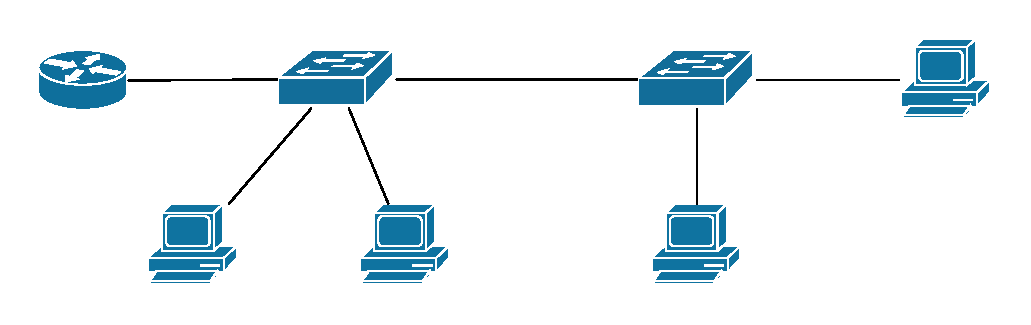
\includegraphics[width=\textwidth]{generic-topology}
	\caption{H γενική άποψη της τοπολογίας προς υλοποίηση.}\label{fig:generic-topoloy}
\end{figure}

Για την υλοποίηση της τοπολογίας θα χρειαστείτε τις εξής συσκευές:

\begin{itemize}
	\item x2 δρομολογητές Cisco 2921
	\item x2 δρομολογητές MikroTik CCR-1009
	\item x1 μεταγωγέας Cisco (μόνο για το πρώτο σενάριο)
	\item x1 υπολογιστή
\end{itemize}

\section{Θεωρητικό υπόβαθρο}
To OSPF (Open Shortest Path First) αποτελεί ένα ανοιχτό πρωτόκολλο δρομολόγησης εσωτερικής πύλης (\textbf{IGP}), το οποίο ανήκει στην κατηγορία των \textbf{πρωτοκόλλων δρομολόγησης με κατάσταση συνδέσμων} (link-state routing protocol).

Κύριο χαρακτηριστικό των πρωτοκόλλων κατάστασης συνδέσμων είναι πως η σύγκλιση επιτυγχάνεται με ανταλλαγή διαφημίσεων, στις οποίες ο κάθε δρομολογητής περιλαμβάνει πληροφορίες για τους γειτονικούς του δρομολογητές. Οι δρομολογητές που βρίσκονται σε ένα συγκεκριμένο εύρος, δηλαδή στην ίδια περιοχή, συλλέγουν τα εν λόγω πακέτα και διαμορφώνουν έναν χάρτη, ο οποίος αποτυπώνει την λογική τοπολογία. Μετά από ένα συγκεκριμένο χρονικό διάστημα, ο κάθε δρομολογητής εφαρμόζει στον χάρτη που έχει κατασκευάσει τον αλγόριθμο ελάχιστου μονοπατιού του Dijkstra (Shortest Path First - SPF) για να υπολογίσει τη συντομότερη διαδρομή προς κάθε δρομολογητή/προορισμό και να ενημερώσει κατάλληλα τον πίνακα δρομολόγησής του. 

Η λειτουργία των πρωτοκόλλων κατάστασης συνδέσμων διαφέρει σημαντικά από αυτή των πρωτοκόλλων δρομολόγησης με διανύσματα απόστασης (distance vector). Στον πίνακα \ref{tab:comparison} παρατίθενται συνοπτικά αυτές οι διαφορές. Επισημαίνεται ότι η σύγκριση αφορά περισσότερο τη λειτουργία των πρωτοκόλλων OSPF και RIP, παρά μια γενικότερη σύγκριση μεταξύ των δυο κατηγοριών. Για παράδειγμα, πιο περίπλοκα πρωτόκολλα διανυσμάτων απόστασης, όπως το EIGRP, αν και δεν ανήκει στην κατηγορία των πρωτοκόλλων κατάστασης συνδέσμων, ωστόσο διατηρεί πολλά πλεονεκτήματά τους, όπως η δημιουργία βάσης δεδομένων με την τοπολογία του δικτύου, η χρήση περιοχών και η χρήση ποιοτικότερων μετρικών για τη διαμόρφωση του πίνακα δρομολόγησης. 

\begin{table}[ht]\renewcommand\arraystretch{1.35}\small
	\centering	\rowcolors{2}{lightgray}{white}
	\begin{tabular}{>{\centering}m{3cm}m{6cm}m{6.5cm}}\FormatFirstRow
											& \textbf{RIP} (distance-vector)		& \textbf{OSPF} (link-state) 				\\
		\textbf{Μεταδιδόμενη πληροφορία}	& Διαδρομές που συμμετέχουν στο RIP.	& Πληροφορίες σχετικά με τους γειτονικούς δρομολογητές (LSA)		\\
		\textbf{Πηγή πληροφορίας}		& Βασίζεται στη φήμη (rumor), δηλαδή σε άλλους πίνακες δρομολόγησης. & Οι διαφημίσεις LSA\\
		\textbf{Γνώση της τοπολογίας}		& Όχι									& Ναι, διατηρείται σχετική βάση δεδομένων (LSDB)	\\
		\textbf{Πολυπλοκότητα λειτουργίας}	& Χαμηλή								& Υψηλότερη, πολλά είδη μηνυμάτων και είδη πακέτων.				\\
		\textbf{Χρησιμοποίηση πόρων}		& Χαμηλή								& Υψηλή, για τη μετάδοση των LSA και τον υπολογισμό του SPT.						\\
		\textbf{Έκταση λειτουργίας}			& Μέχρι 15 άλματα						& Προσαρμόσιμη, ορίζονται περιοχές\\
		\textbf{Μετρική κόστους}			& Πλήθος αλμάτων						& Αθροιστικό εύρος ζώνης\\
		\textbf{Αλγόριθμος}					& Bellman-Ford							& Dijkstra
	\end{tabular}
	\caption{Σύγκριση χαρακτηριστικών δυναμικής και στατικής δρομολόγησης.}\label{tab:comparison}
\end{table}

Το πρωτόκολλο που μελετάτε σε αυτό το φυλλάδιο ορίζεται από το έγγραφο \href{https://tools.ietf.org/html/rfc2328}{RFC 2328} (OSPFv2 για IPv4).
Επίσης, τμήματα της εργαστηριακής άσκησης αναφέρονται στο \href{https://tools.ietf.org/html/rfc3101}{RFC 3101}, το οποίο ορίζει τις περιοχές NSSA, μια προαιρετική επέκταση του OSPF.

Στο παρόν φυλλάδιο δεν θα ασχοληθείτε με το \href{https://tools.ietf.org/html/rfc5340}{RFC 5340} που ορίζει το OSPFv3 για IPv6. Ακόμη, πλήθος βελτιώσεων σε μορφή RFC που έχει δημοσιευτεί για τα βασικά πρότυπα, τα οποία προσθέτουν χαρακτηριστικά ασφαλείας, όπως η κρυπτογράφηση, καθώς και διάφορες λειτουργικές προεκτάσεις, επίσης δεν είναι αντικείμενο του παρόντος φυλλαδίου. 

\subsection{Χαρακτηριστικά του OSPF}

Για κάθε διεργασία OSPF που εκτελεί ένας δρομολογητής, διατηρούνται οι εξής δομές/βάσεις δεδομένων (ΒΔ):~
\begin{itemize}
	\item \textbf{Adjacency Database}: Η βάση περιέχει πληροφορίες για τους γείτονες που έχει ανακαλύψει ο δρομολογητής, οι οποίοι θα πρέπει επίσης να έχουν ενεργοποιήσει το OSPF. Κάθε δρομολογητής σε μια τοπολογία OSPF θα πρέπει να έχει διαφορετικά δεδομένα στη ΒΔ γειτνίασης. 
	\item \textbf{Link-State DataBase - LSDB}: Η βάση περιέχει πληροφορίες για όλους τους δρομολογητές που έχουν ανακαλυφθεί από το OSPF. Τα δεδομένα του πίνακα αναπαριστούν τη δικτυακή τοπολογία. Όλοι οι δρομολογητές μιας περιοχής πρέπει να έχουν τα ίδια δεδομένα στην LSDB, ώστε να θεωρηθεί ότι το OSPF έχει συγκλίνει.
	\item \textbf{OSPF Routing Information Base - OSPF RIB}: Η βάση περιέχει τις διαδρομές που προέκυψαν από την εκτέλεση του αλγορίθμου Dijkstra στην LSDB ή από διαδρομές που λαμβάνονται από LSA. Τα περιεχόμενα της βάσης προστίθενται στον καθολικό RIB, δηλαδή τον πίνακα δρομολόγησης.
\end{itemize}

Κάθε καταχώριση της LSDB χαρακτηρίζεται από ένα μοναδικό αναγνωριστικό του γείτονα (router ID), το αντίστοιχο αναγνωριστικό του δρομολογητή από τον οποίο διαφημίστηκε η καταχώριση, η ηλικία της καταχώρισης και το κόστος μετάβασης. 

Αν για έναν προορισμό προκύπτουν πολλές διαδρομές, τo κόστος μετάβασης καθορίζει τη διαδρομή που θα εγκατασταθεί στον πίνακα δρομολόγησης. Για κάθε μια διεπαφή OSPF ενός δρομολογητή ορίζεται ένα κόστος διάσχισης. Το OSPF υπολογίζει το συνολικό κόστος ή μετρική (metric) για κάθε μια διαδρομή, αθροίζοντας το κόστος διάσχισης κάθε διεπαφής εξόδου (egress interface) που χρησιμοποιείται μέχρι τον προορισμό.

Οι δρομολογητές που εκτελούν το OSPF μεταδίδουν πολλά είδη μηνυμάτων. Τα πακέτα αυτά ενθυλακώνονται ως ωφέλιμη πληροφορία της κεφαλίδας IP με τον κωδικό πρωτοκόλλου 89. Τα είδη των μηνυμάτων OSPF παρατίθενται στον πίνακα \ref{tab:messages}. H γενική μορφή ενθυλάκωσης ενός μηνύματος OSPF φαίνεται στο σχήμα \ref{fig:encapsulation}.

\begin{table}[ht]\renewcommand\arraystretch{1.35}\small
	\centering	\rowcolors{2}{lightgray}{white}
	\begin{tabular}{>{\centering}lm{3cm}m{4cm}m{4.0cm}m{3cm}}\FormatFirstRow
\textbf{Type}	& \textbf{Πακέτο}							 & \textbf{Περιγραφή}  										& \textbf{Περιεχόμενα} 										 & \textbf{Προορισμός}		\\
		1		& \textbf{Hello} 							 & Ανακαλύπτει γείτονες, χτίζει και διατηρεί γειτνιάσεις	& Βλ. σχήμα \ref{fig:encapsulation}							 & 224.0.0.5	\\
		2		& Database Descriptor (\textbf{DBD})		 & Συνοψίζει την LSDB								    	& MTU της διεπαφής, αριθμό ακολουθίας του DBD, κεφαλίδες LSA & 224.0.0.5 ή 224.0.0.6 \\
		3		& Link-State Request (\textbf{LSR})			 & Ζητά ένα ή περισσότερα πλήρη LSA							& Κεφαλίδες LSA												 & Unicast (αποστολέας του DBD) \\
		4		& Link-State Update (\textbf{LSU})			 & Απαντά σε ένα LSU										& Πλήρη LSA													 & 224.0.0.5 ή 224.0.0.6 \\
		5		& Link-State Acknowledgment (\textbf{LSAck}) & Επιβεβαιώνει τη λήψη LSU 								& Κεφαλίδες LSA 											& Unicast ή 224.0.0.5 ή 224.0.0.6
	\end{tabular}
	\caption{Τα είδη μηνυμάτων OSPF.}\label{tab:messages}
\end{table}

\begin{figure}[ht]
	\centering
	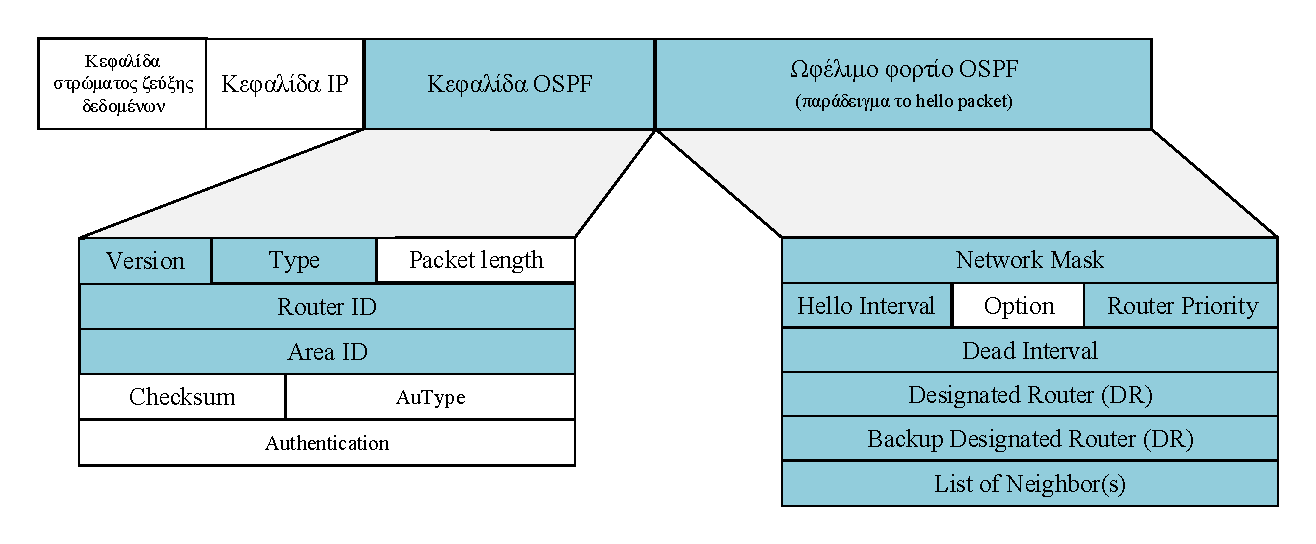
\includegraphics[width=\textwidth]{encapsulation}
	\caption{Η ενθυλάκωση OSPF με παράδειγμα το μήνυμα Hello.}\label{fig:encapsulation}
\end{figure}

Τα σημαντικότερα πεδία που διαμορφώνουν την κεφαλίδα OSPF συνοψίζονται στα εξής: 
\begin{itemize}
	\item \textbf{Version}: H έκδοση του OSPF που χρησιμοποιείται (πχ OSPFv2).
	\item \textbf{Type}: To είδος του μηνύματος που περιέχεται ως ωφέλιμο φορτίο OSPF  (στήλη πίνακα \ref{tab:messages}).
	\item \textbf{Router ID}\label{router-id}: Είναι ένας αριθμός 32 bit, που αναγράφετραι σε μορφή διεύθυνσης IPv4, και αναπαριστά την ταυτότητα ενός δρομολογητή στο OSPF. Το Router ID πρέπει να είναι μοναδικό μέσα σε ένα AS. Ο μηχανισμός επιλογής Router ID εξαρτάται από το λειτουργικό σύστημα. Το \textbf{Cisco IOS} επιλέγει το Router ID με βάση τα εξής κριτήρια
	\begin{enumerate}
		\item Χειροκίνητος ορισμός από το CLI 
		\item Αν δεν έχει οριστεί από το CLI, τότε επιλέγεται η μεγαλύτερη διεύθυνση IP που έχει ανατεθεί σε διεπαφή βρόχου (loopback).
		\item Αν δεν υπάρχει διεπαφή βρόχου, επιλέγεται η μεγαλύτερη διεύθυνση IP που έχει ανατεθεί σε οποιαδήποτε άλλη διεπαφή. 
	\end{enumerate}
	Αντίθετα, στο \textbf{RouterOS}, αν δεν έχει οριστεί χειροκίνητα το Router ID, τότε επιλέγεται η μικρότερη διεύθυνση IP που έχει ανατεθεί σε οποιαδήποτε διεπαφή.
	\item \textbf{Area ID}: H περιοχή στην οποία ανήκει η διεπαφή του δρομολογητή, από την οποία παρήχθη το πακέτο.
\end{itemize}

Αντίστοιχα για το μήνυμα Hello, τα σημαντικότερα πεδία είναι τα εξής:
\begin{itemize}
	\item \textbf{Network Mask}: H μάσκα του δικτύου στο οποίο ανήκει η διεπαφή που στέλνει το μήνυμα.
	\item \textbf{Hello interval}: Η περίοδος αποστολής μηνυμάτων hello. Δυο δρομολογητές με διαφορετικά hello interval δεν μπορούν να χτίσουν γειτνίαση. Προεπιλεγμένη τιμή είναι τα 10 δευτερόλεπτα για ethernet και point-to-point και 30 δευτερόλεπτα για δίκτυα ΝΒΜΑ\footnote{Non-Broadcast Multiple Aceess (ΝΜΒΑ): Είναι τα τηλεπικοινωνιακά δίκτυα πολλαπλής πρόσβασης, στα οποία δεν επιτρέπονται οι ευρυεκπομπές.}.
	\item \textbf{Router priority}: Αριθμός που καθορίζει την προτεραιότητα ενός δρομολογητή στην εκλογή DR/BDR.
	\item \textbf{Dead interval}: Αν μετά την πάροδο αυτού του χρόνου δεν ληφθεί πακέτο hello από κάποιον γείτονα, τότε αυτός διαγράφεται από τις ΒΔ. Προεπιλεγμένη του τιμή είναι 4 φορές το hello time.
	\item \textbf{DR}/\textbf{BDR}: Για κάθε ζεύξη πολλαπλής πρόσβασης (πχ ethernet) ορίζεται ένας δρομολογητής DR και ένας BDR. Στο πακέτο hello περιλαμβάνεται το router ID των δρομολογητών με αυτούς τους ρόλους.
	\item \textbf{List of Neighbor(s)}: Στο πεδίο αυτό ο δρομολογητής συμπεριλαμβάνει τα router ID των γειτόνων του. 
\end{itemize}

\subsection{Στάδια εγκαθίδρυσης γειτνίασης}

H ολοκλήρωση της γειτνίασης δυο δρομολογητών, με αποτέλεσμα τη σύγκλιση των LSDB τους, επιτυγχάνεται μέσα από τη μετάβαση 7 καταστάσεων (OSPF States). Οι καταστάσεις χωρίζονται σε δυο φάσεις, τη φάση ανακάλυψης γειτόνων και τη φάση συγχρονισμού των LSDB. Στην τελευταία κατάσταση, οι γειτονικοι δρομολογητές έχουν εγκαθιδρύσει πλήρη γειτνίαση και οι LSDB τους είναι ίδιες. Όταν όλοι οι δρομολογητές ενός δικτύου OSPF είναι στην τελευταία κατάσταση, τότε το δίκτυο έχει συγκλίνει. Οι εν λόγω καταστάσεις παρατίθενται στο σχήμα \ref{fig:states}.

\begin{figure}[ht]
	\centering
	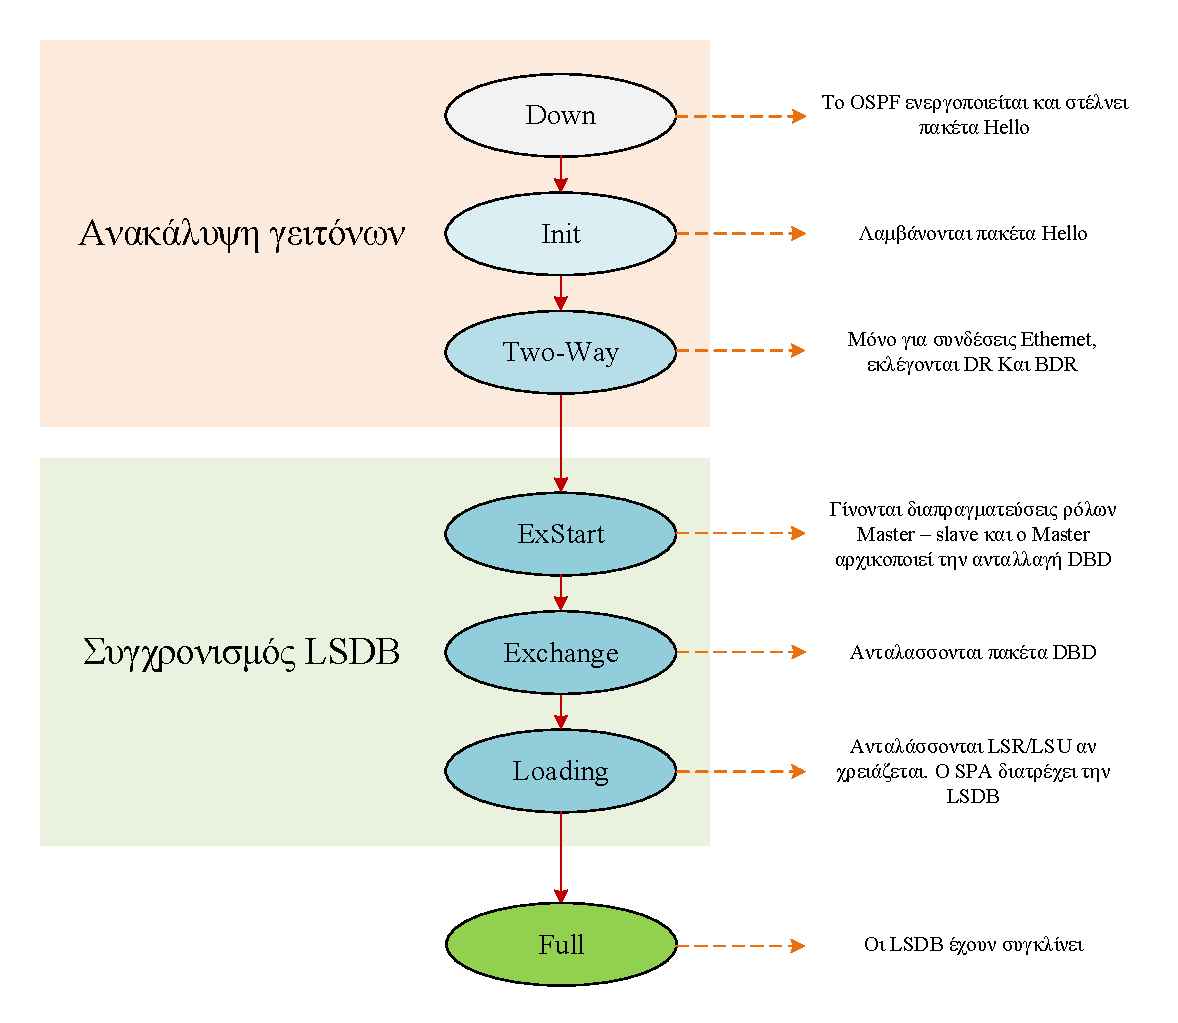
\includegraphics[width=\textwidth]{states}
	\caption{Οι καταστάσεις OSPF.}\label{fig:states}
\end{figure}

Πρώτο βήμα της διαδικασίας είναι η κατάσταση \textbf{Down}, κατά την οποία ο δρομολογητής στέλνει μηνύματα Hello μέσω όλων των διεπαφών που συμμετέχουν στο OSPF. 

Δεύτερο βήμα είναι η κατάσταση \textbf{Init}, στην οποία εισέρχεται ο δρομολογητής όταν λάβει το πρώτο μήνυμα Hello από κάποιον γείτονα. Ο δρομολογητής διαβάζει το πεδίο router ID της κεφαλίδας OSPF και, αν πληρούνται ορισμένα κριτήρια, προσθέτει τον γειτονικό δρομολογητή στη λίστα γειτόνων του. Στα επόμενα μηνύματα hello που στέλνει ο δρομολογητής συμπεριλαμβάνει στο πεδίο List of Neighbor(s) τα router ID των γειτόνων που πρόσθεσε.

\warningbox{Για να συμπεριληφθεί ένας δρομολογητής σε μια λίστα γειτόνων θα πρέπει πρέπει στις γειτονικές διεπαφές των δυο δρομολογητών να ταυτίζεται το hello interval, το dead interval, το area ID, οι σημαίες stub area και η ταυτότητα δικτύου. Αν δεν ταυτίζεται κάτι από τα παραπάνω, τότε δεν εγκαθιδρύεται γειτνίαση.}

Αν ένας δρομολογητής αναγνωρίσει το δικό του router ID σε ένα πακέτο hello και η διεπαφή από την οποία το λαμβάνει είναι τύπου ethernet ή NBMA, τότε εισέρχεται σε κατάσταση \textbf{Two-Way} και διεξάγει εκλογή DR/BDR. H εκλογή περιγράφεται στην υποενότητα \ref{sec:dr}. Αν η ζεύξη δεν είναι ethernet ή NBMA, τότε ο δρομολογητής μεταβαίνει στην κατάσταση ExStart.

Στην κατάσταση \textbf{ExStart}, για κάθε γειτνίαση, αποφασίζεται ποιος δρομολογητής θα είναι ο master, δηλαδή αυτός που θα στείλει πρώτος το DBD της βάσης του. Για να ληφθεί αυτή η απόφαση, ο κάθε δρομολογητής στέλνει στον γειτονικό του ένα άδειο DBD με τις σημαίες Init και master ενεργοποημένες. Ο δρομολογητής, βλέποντας τις εν λόγω σημαίες ενεργοποιημένες, αποφασίζει αν θα είναι ο ίδιος ή ο γείτονάς του master συγκρίνοντας τα router ID, με το υψηλότερο router ID να προηγείται στην εκλογή. Αφού αναδειχθεί ο master, τότε αυτός αρχικοποιεί το πρώτο DBD και ξεκινά η μετάβαση στην κατάσταση Exchange.

\warningbox{Αν μια διεπαφή λάβει DBD με διαφορετικό MTU από το δικό της (βλ. πίνακα \ref{tab:messages} για τα περιεχόμενα του DBD), τότε η διαδικασία «παγώνει» στο στάδιο ExStart.}

Ο δρομολογητής της κατάστασης \textbf{Exchange} στέλνει και λαμβάνει πακέτα DBD. Ο δρομολογητής συγκρίνει τις κεφαλίδες LSA που λαμβάνει με τα περιεχόμενα της LSDB. Αν βρεί πως του λείπει κάποια καταχώριση είτε η καταχώριση δεν είναι ενημερωμένη, τότε η γειτνίασή του μεταβαίνει στην κατάσταση Loading.

Στην κατάσταση \textbf{Loading}, ο δρομολογητής στέλνει LSR, συμπεριλαμβάνοντας τις κεφαλίδες LSA που χρειάζονται ενημέρωση. Ως απάντηση, λαμβάνει LSU με τα πλήρη LSA που ζήτησε. Εκτός του ότι ενημερώνει τη LSDB με τα νέα LSA, ο δρομολογητής συσκευάζει τα LSA σε νέα LSU, τα οποία διαχέει (floods) προς συγκεκριμένες διεπαφές. Εξαρτάται από το είδος του LSA οι διεπαφές που θα επιλεγούν για τη διάχυση. Όταν πλέον τα DBD είναι ταυτόσημα με τις LSDB, τότε οι δρομολογητές μεταβαίνουν στην κατάσταση Full, κατά την οποία έχει επιτευχθεί σύγκλιση. 

Κατά τη διάρκεια της κατάστασης \textbf{Full}, συνεχίζεται η ανταλλαγή μηνυμάτων Hello κάθε hello time. Από την κατάσταση αυτή ενδέχεται ένας δρομολογητής να επιστρέψει στην κατάσταση Loading, αν λάβει LSU. Ο δρομολογητής μπορεί να στείλει LSU αν συμβεί κάτι από τα εξής:~
\begin{itemize}
	\item Δεν λάβει πακέτο hello μετά από χρόνο dead interval και αφαιρέσει τον γείτονα από την LSDB.
	\item Αποτύχει κάποια διεπαφή που συμμετέχει στο OSPF.
	\item Όταν περάσουν 30 λεπτά χωρίς να έχει δημιουργήσει κάποιο LSU. Κάθε δρομολογητής πρέπει το πολύ κάθε 30 λεπτά να παράγει και να διαχέει LSA στο δίκτυο, ακόμη και αν δεν έχει συμβεί κάποια αλλαγή.
\end{itemize}

\subsection{OSPF και δίκτυα πολλαπλής πρόσβασης}\label{sec:dr}

H δημιουργία γειτνιάσεων OSPF σε δίκτυα πολλαπλής πρόσβασης χρειάζεται ιδιαίτερη προσοχή. Αν $N$ δρομολογητές είναι συνδεδεμένοι σε έναν μεταγωγέα και έχουν ενεργοποιήσει όλοι το OSPF, σύμφωνα με τη διαδικασία εγκαθίδρυσης γειτνιάσεων που περιγράφηκε, θα έπρεπε κάθε δρομολογητής να εγκαθιδρύσει γειτνίαση με κάθε άλλο δρομολογητή που συνδέεται στον μεταγωγέα. Οι γειτνιάσεις του τομέα ευρυεκπομπής θα ήταν ${N(N-1)/2}$ και οι δρομολογητές θα αντάλλασσαν $N^2$ φορές περισσότερα μηνύματα.

H εγκαθίδρυση τόσων γειτνιάσεων είναι περιττή και δημιουργεί αυξημένη επιβάρυνση με αποστολές LSA. Το OSPF φροντίζει για την απάλειψη των περιττών γειτνιάσεων σε ένα δίκτυο πολλαπλής πρόσβασης με την εκλογή ενός δρομολογητή με τον ρόλο \textbf{Designated Router} (DR). Ως εφεδρικός του DR εκλέγεται ο δεύτερος στη σειρά εκλογής με τον ρόλο του \textbf{Backup Designated Router} (DBR) και αναδεικνύεται ως DR αυτόματα, όταν ο DR αποτύχει. Οι δρομολογητές που δεν είναι ούτε DR ούτε BDR αποκαλούνται DROTHER.

O DR είναι το διακομετακομιστικό μέσο των LSΑ, δηλαδή λαμβάνει και αποστέλλει ενημερώσεις εκ μέρους των υπολοίπων δρομολογητών. Για παράδειγμα, ο δρομολογητής που θέλει να στείλει ένα LSA στους γείτονές του, στέλνει το πακέτο στον DR και ο DR το στέλνει στη συνέχεια σε όλους τους υπόλοιπους δρομολογητές. Για την επικοινωνία των DROTHER με τους DR/BDR χρησιμοποιείται η διεύθυνση πολυεκπομπής 224.0.0.6. 

Κριτήρια για την εκλογή DR/BDR είναι τα εξής, με σειρά προτίμησης:
\begin{enumerate}
	\item Ο δρομολογητής με την υψηλότερη προτεραιότητα (router priority). Προεπιλεγμένη τιμή είναι το 1. Δρομολογητής με προτεραιότητα 0 αποκλείεται από τη διαδικασία εκλογής και η τιμή 255 είναι η μέγιστη δυνατή προτεραιότητα.
	\item Αν οι προτεραιότητες είναι ίδιες, τότε αναδεικνύεται αυτός με το υψηλότερο router ID. H επιλογή του router ID περιγράφεται στη σελίδα \pageref{router-id}.
\end{enumerate}

\subsection{OSPF πολλαπλών περιοχών}\label{multiple-areas}

Το OSPF μπορεί να επιβαρύνει σημαντικά ένα δίκτυο, όταν πολλοί δρομολογητές βρίσκονται στο ίδιο AS (Autonomous System) και στην ίδια περιοχή. Συγκεκριμένα, σε μια τέτοια περίπτωση: \begin{enumerate*}[label=\alph*)] \item μεγαλώνει σημαντικά ο πίνακας δρομολόγησης του καθενός \item μεγαλώνουν σημαντικά οι LSDB \item εκτελείται συχνότερα ο SPF στην ήδη μεγάλη LSDB και \item καταναλώνεται περισσότερο εύρος ζώνης για την προώθηση LSA.
\end{enumerate*}
%
%καθώς και τις πληροφορίες που αποκτούν για αυτή την περιοχή δρομολογητές που βρίσκονται εκτός αυτής

Το OSPF αντιμετωπίζει αυτά τα προβλήματα με τον χωρισμό ενός AS σε \textbf{περιοχές} (areas). Η μετάδοση των LSA περιορίζεται μέσα στις περιοχές, ενώ μεταξύ των περιοχών ανταλλάσσονται άλλα είδη LSA, τα οποία διαφημίζουν διαδρομές και δεν προκαλούν εκτέλεση του STP. Ο περιορισμός της πληροφορίας που διακινείται εξοικονομεί εύρος ζώνης, περιορίζει το μέγεθος των πινάκων δρομολόγησης και των LSDB, αλλά και μειώνει τη συχνότητα εκτελέσεων του SPF.

Υπάρχουν δυο βασικά είδη περιοχών, η \textbf{κορμού} ή μεταβιβαστική (backbone, transit) που εξυπηρετεί την επικοινωνία μεταξύ διαφορετικών περιοχών και οι \textbf{κανονικές} (regular, non-backbone). Κάθε περιοχή προσδιορίζεται από έναν αριθμό 32 bit, ο οποίος εμφανίζεται στην κεφαλίδα OSPF. Οι περιοχές εφαρμόζονται σε επίπεδο διεπαφής, δηλαδή μια διεπαφή (άρα και το δίκτυο που της έχει ανατεθεί) πρέπει να ανήκει σε μια περιοχή. Μια διεπαφή μπορεί να ανήκει σε μια μόνο περιοχή, αλλά ένας δρομολογητής μπορεί να ανήκει σε πολλές περιοχές. Από προεπιλογή, κάθε διεπαφή ανήκει στην περιοχή 0, η οποία είναι η περιοχή κορμού. 

Ανάλογα με τη συμμετοχή τους σε περιοχές, οι δρομολογητες OSPF κατατάσσονται στις εξής κατηγορίες:
\begin{itemize}
	\item \textbf{Internal Router}: Είναι ο δρομολογητής, του οποίου οι διεπαφές βρίσκονται όλες σε στην ίδια περιοχή.
	
	\item \textbf{Backbone Router}: Είναι ο δρομολογητής, του οποίου οι διεπαφές (όχι απαραίτητα όλες) βρίσκονται στην περιοχή κορμού.
	
	\item \textbf{Area Border Router} (ABR): Είναι ο δρομολογητής, του οποίου οι διεπαφές βρίσκονται ταυτόχρονα σε διαφορετικές περιοχές. Ένας ABR διατηρεί ξεχωριστές LSDB για κάθε περιοχή στην οποία είναι συνδεδεμένος. Ρόλος του είναι να διασυνδέει κανονικές περιοχές με την περιοχή κορμού, να διαφημίζει τα δίκτυα των περιοχών που εξυπηρετεί στο δίκτυο κορμού και τους υπόλοιπους ABR (και προαιρετικά να τα συναθροίζει), καθώς και να εισάγει στις περιοχές που εξυπηρετεί προθέματα που διαφημίζονται από άλλους ABR.
	
	\item \textbf{Autonomous System Boundary Router} (ASBR): Είναι ο δρομολογητής που διαθέτει τουλάχιστον μια διεπαφή συνδεδεμένη σε ένα εξωτερικό δίκτυο. Το δίκτυο αυτό μπορεί να είναι κάποιο που εκτελεί διαφορετικό πρωτόκολλο δρομολόγησης IGP ή κάποιο που ανήκει σε διαφορετικό AS και εκτελεί BGP για την επικοινωνία μεταξύ AS. Ρόλος του ASBR είναι να εξυπηρετεί την επικοινωνία του δικτύου OSPF με εξωτερικά δίκτυα, να εισάγει εξωτερικές διαδρομές αλλά και να εξάγει προθέματα, τα οποία μπορεί προαιρετικά να συναθροίζει.
\end{itemize}

Η αρχιτεκτονική σχεδιασμού περιοχών πρέπει να ακολουθεί τους εξής κανόνες:
\begin{itemize}
	\item Μια περιοχή δεν μπορεί να έχει πάνω από 50 δρομολογητές.
	\item Ένας δρομολογητής δεν μπορεί να είναι ταυτόχρονα σε πάνω από 3 περιοχές.
	\item Ένας δρομολογητής δεν μπορεί να έχει πάνω από 60 γείτονες.
	\item Όλες οι περιοχές πρέπει να συνδέονται απευθείας με την περιοχή κορμού. Αν αυτό δεν είναι δυνατό, χρησιμοποιείται η τεχνική των virtual link. 
	\item Κίνηση που προορίζεται προς διαφορετικές περιοχές, πρέπει να διέρχεται από την περιοχή κορμού.
\end{itemize}

\notebox{Οι διαδρομές που προκύπτουν μετά από εκτέλεση του SPF σε μια περιοχή, δε μπορούν να προκαλέσουν βρόχους (routing loops). Ωστόσο, μεταξύ διαφορετικών περιοχών OSPF εφαρμόζεται μηχανισμός δρομολόγησης διανυσμάτων απόστασης, αφού η επικοινωνία μεταξύ περιοχών βασίζεται σε διαφήμιση προθεμάτων, και έτσι ελλοχεύει κίνδυνος δημιουργίας βρόχων. Για να αποφευχθούν οι βρόχοι μεταξύ περιοχών, η κίνηση μεταξύ διαφορετικών περιοχών πρέπει οπωσδήποτε να εξυπηρετείται από το δίκτυο κορμού. Για περισσότερες λεπτομέρειες μπορείτε να ανατρέξετε στο εξής άρθρο: \url{https://www.networkworld.com/article/2348778/cisco-subnet/my-favorite-interview-question.html}}

\subsection{Κατηγοριοποίηση των LSA και είδη διαδρομών OSPF}

Ένας από τους λόγους για τους οποίους χρησιμοποιούνται οι περιοχές OSPF είναι για να περιορίζουν τη διάδοση των LSA. To OSPF διατηρεί 11 διαφορετικά είδη LSA, τα οποία εξυπηρετούν αυτόν τον σκοπό και έχουν ως εξής:\footnote{Έχουν παραληφθεί οι τύποι 6, 8, 9-11 που αφορούν κατά αντιστοιχία το Multicast OSPF, το OSPFv3 και τα διαφανή LSA.}. Βασικό πεδίο κάθε είδους LSA είναι το Link State ID, το οποίο εμφανίζεται στην LSDB και έχει διαφορετική ερμηνεία για κάθε είδος LSA.

\begin{itemize}
	\item [Type 1:] \textbf{Router LSA} -- Κάθε δρομολογητής στέλνει ένα τέτοιο πακέτο για να διαφημίσει τις διεπαφές OSPF που έχει, το κόστος της κάθε διεπαφής, καθώς και τον ρόλο του (ABR ή ASBR). Το πεδίο Link State ID συνήθως περιγράφει το router ID του γείτονα ή την IP του DR. Το πακέτο αυτό δεν προωθείται εκτός της περιοχής από την οποία παρήχθη.
	
	\item [Type 2:] \textbf{Network LSA} -- Είναι οι διαφημίσεις που στέλνει μόνο ο DR σε ένα δίκτυο πολλαπλής πρόσβασης. Στη διαφήμιση περιλαμβάνεται η μάσκα υποδικτύου και router ID όλων των δρομολογητών που συμμετέχουν στο ίδιο δίκτυο. Το πεδίο Link State ID περιέχει τη διεύθυνση IP της διεπαφής του DR. Το πακέτο δεν προωθείται εκτός της περιοχής από την οποία παρήχθη. 
	
	\item [Type 3:] \textbf{Summary LSA} -- Κάθε ABR στέλνει ένα τέτοιο πακέτο για να διαφημίσει διαδρομές που έμαθε από τα LSA τύπου 1. Για κάθε απομακρυσμένο δίκτυο περιλαβάνει την ταυτότητα δικτύου και το κόστος μέχρι τον ABR. Το πεδίο Link State ID περιέχει την ταυτότητα του δικτύου που διαφημίζεται. Τα πακέτα αυτά διαδίδονται σε όλο το δίκτυο OSPF μέσω των ABR. 
	
	\item [Type 4:] \textbf{ASBR-Summary LSA} -- Είναι ίδια με την Summary LSA, αλλά διαφημίζει διαδρομές προς τον ή τους ASBR του δικτύου. Το Link State ID αυτού του πακέτου περιέχει το router ID του ASBR που διαφημίζεται.
	
	\item [Type 5:] \textbf{AS External LSA} -- Οι ASBR παράγουν τέτοια πακέτα για να διαφημίσουν διαδρομές για προορισμούς εκτός του δικτύου OSPF. Το Link State ID περιέχει την ταυτότητα του δικτύου που διαφημίζεται. Στην περίπτωση που διαφημίζεται η προεπιλεγμένη πύλη, η τιμή του πεδίου είναι 0.0.0.0. Τα πακέτα αυτά διαχέονται από τους ABR σε όλο το δίκτυο OSPF. 
	
	\item [Type 7:] \textbf{NSSA LSA} -- Είναι το ειδικό πακέτο LSA που εξυπηρετεί τη λειτουργία περιοχών NSSA. Ένα πακέτο τύπου 7 δημιουργείται αποκλειστικά από ASBR που βρίσκεται σε περιοχή NSSA και μετατρέπεται σε LSA τύπου 5 από τους ABR που το λαμβάνουν.  
\end{itemize}

\notebox{Τα LSA 3, 4, 5 και 7 αποτελούν διαφημίσεις διαδρομών. Αυτό σημαίνει ότι προστίθενται στην LSDB και στον πίνακα δρομολόγησης χωρίς να προκαλούν επανεκτέλεση του SFP.}

Κάθε είδος LSA συνοδεύεται από μια κεφαλίδα LSA, η οποία είναι η ίδια που μεταδίδεται και σε όλα τα άλλα είδη μηνυμάτων OSPF (βλ πίνακα \ref{tab:messages}). Τα περιεχόμενά της έχουν ως εξής:

\begin{itemize}
	\item \textbf{LS age}: Η ηλικία παραγωγής του LSA σε δευτερόλεπτα.
	\item \textbf{LS type}: Το είδος του LSA.
	\item \textbf{Link State ID}: Εξαρτάται από το είδος του μηνύματος LSA.
	\item \textbf{Advertising Router}: To router ID του δρομολογητή που παρήγαγε το πρωτότυπο LSA.
	\item \textbf{LS sequence number}: Για τον εντοπισμό παλιών ή διπλότυπων LSA.
\end{itemize}

Υπάρχουν περιπτώσεις στις οποίες δεν είναι επιθυμητή η διάχυση διαδρομών σε συγκεκριμένες περιοχές. Για παράδειγμα, δεν χρειάζεται οι δρομολογητές που βρίσκονται σε δίκτυα-απολήξεις (stub networks) να έχουν καταχωρήσεις για κάθε μια εξωτερική διαδρομή, αλλά μια προεπιλεγμένη πύλη που να οδηγεί στα εξωτερικά δίκτυα. Το OSPF ορίζει τα εξής είδη περιοχών ως υποκατηγορίες των περιοχών non-backbone:
\begin{itemize}
	\item \textbf{Stub area}: Στην περιοχή επιτρέπεται η προώθηση LSA τύπου 1, 2, 3 και 4, ενώ οι διαφημίσεις τύπου 5 αντικαθίστανται από μια διαφήμιση προεπιλεγμένης πύλης. Η προεπιλεγμένη πύλη αφορά μόνο τους προορισμούς εκτός δικτύου OSPF.  
	\item \textbf{Totally stubby area}: Eπιτρέπεται μόνο η προώθηση LSA τύπου 1 και 2, καθώς και ένα LSA τύπου 3 που διαφημίζει την προεπιλεγμένη πύλη. Η προεπιλεγμένη πύλη εξυπηρετεί προορισμούς εκτός της περιοχής αλλά και εκτός του δικτύου OSPF.
	\item \textbf{Not-so-stubby area} (NSSA): Η περιοχή επιτρέπει σε έναν ASBR να διαφημίσει εξωτερικά δίκτυα μέσω της NSSA, χωρίς ταυτόχρονα να επιτρέπεται η διάχυση LSA τύπου 5 στην περιοχή αυτή. Ο ASBR ενθυλακώνει τις διαφημίσεις αυτές σε LSA τύπου 7 για να τις μεταδώσει στην περιοχή NSSA, με τον ABR που βρίσκεται στο απέναντι άκρο της περιοχής να τις μεταφράζει σε τύπου 5 πριν τις διαχύσει περαιτέρω στο δίκτυο.
	\item \textbf{Totally Not-so-stubby area} (Totally NSSA): Το ίδιο με την NSSA, αλλά αφορά τον περιορισμό και των LSA τύπου 3 και 4. 
\end{itemize}

Τέλος, ένας πίνακας δρομολόγησης OSPF διατηρεί τα εξής είδη διαδρομών:
\begin{itemize}
	\item \textbf{Intra-area route} (εσωτερική διαδρομή): Πρόκειται για μια τυπική διαδρομή OSPF που προέκυψε από LSA τύπου 1 και εκτέλεση του OSPF και αφορά προορισμό περιοχής, στην οποία ανήκει ο δρομολογητής. Στους πίνακες δρομολόγησης των συσκευών Cisco, οι διαδρομές αυτές σημειώνονται με \ip{O}.
	
	\item \textbf{Inter-area route} (διαδρομή μεταξύ περιοχών): Πρόκεται για διαδρομές που προέρχονται από περιοχές στις οποίες δεν ανήκει ο δρομολογητής. Στους πίνακες δρομολόγησης των συσκευών Cisco, οι διαδρομές αυτές σημειώνονται με \ip{O IA}. Οι διαδρομές αυτές προέκυψαν από λήψη LSA τύπου 3 ή 4.
	
	\item \textbf{External routes} (εξωτερικές διαδρομές): Πρόκειται για διαδρομές από άλλο AS που εισήλθαν στο δίκτυο μέσω ενός ASBR. Οι διαδρομές αυτές εμφανίζονται στις συσκευές Cisco ως \ip{O E1} ή \ip{O E2} στις κανονικές περιοχές και ως \ip{O N1} ή \ip{O N2} στις NSSA. Οι διαδρομές αυτές προέκυψαν από λήψη LSA τύπου 5 ή 7. Οι εξωτερικές διακρίνονται σε δυο είδη:
	\begin{itemize}
	 \item Τύπου 1: Σε αυτές προστίθεται στο αρχικό κόστος της διαδρομής, το κόστος του μονοπατιού από τον ASBR που τη διαφημίζει μέχρι τον δρομολογητή που τη λαμβάνει. 
	 \item Τύπου 2: Το κόστος της εξωτερικής διαδρομής που εισάγεται, παραμένει ανέπαφο κατά τη διάδοσή της στο δίκτυο OSPF. Όλες οι εξωτερικές διαδρομές είναι από προεπιλογή τύπου 2.  
	\end{itemize}
	\item \textbf{Προεπιλεγμένη διαδρομή OSPF}: H προεπιλεγμένη διαδρομή που διαφημίστηκε από το OSPF. Στους πίνακες δρομολόγησης των συσκευών Cisco, οι διαδρομές αυτές σημειώνονται με \ip{O*IA}.
\end{itemize}

\newpage

\section{Προετοιμασία δικτύου}

\begin{figure}[H]
	\centering
	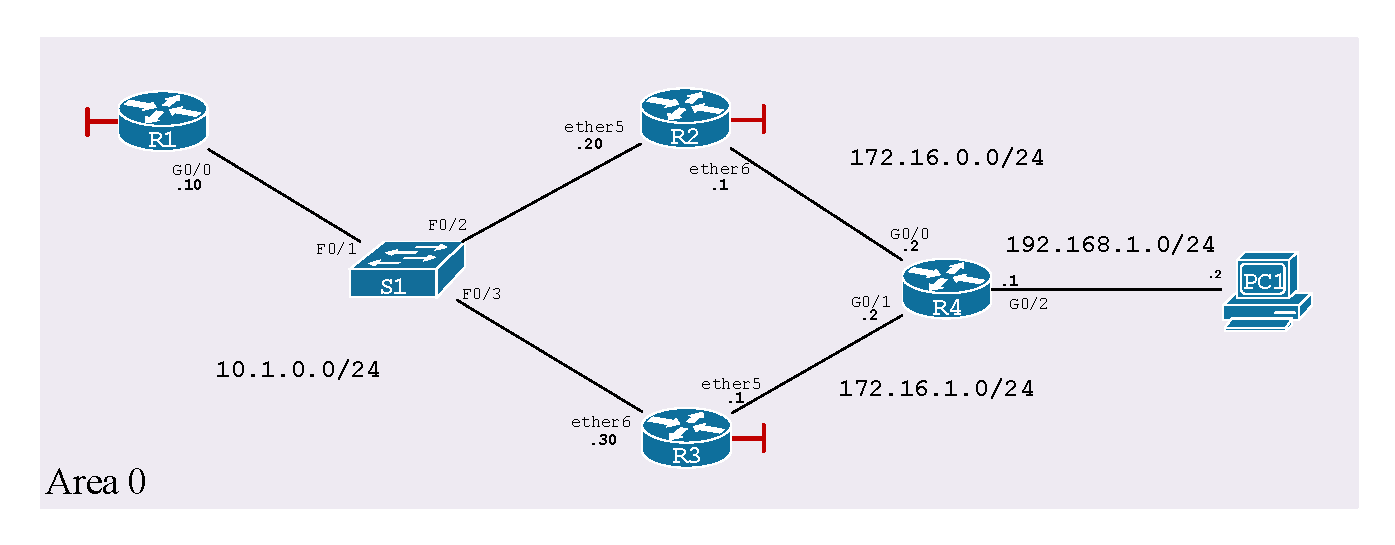
\includegraphics[width=\linewidth]{topology-1}
	\caption{Το σχέδιο της αναλυτικής τοπολογίας προς υλοποίηση.}\label{fig:topology1}
\end{figure}

\begin{IpAddressTable}{Σχήμα διευθυνσιοδότησης της τοπολογίας του πρώτου σεναρίου.}{addr}
							 & Gi0/0		& 10.1.0.10		& 255.255.255.0			&\\
	\multirow{-2}{*}{R1}	 & loopback0	& 1.1.1.1		& 255.255.255.255		&\multirow{-2}{*}{1.1.1.1}\\
	\rowcolor{lightgray}	 & ether5		& 10.1.0.20		& 255.255.255.0 	    &\\
	\rowcolor{lightgray}	 & ether6		& 172.16.0.1	& 255.255.255.0			&\\
	\rowcolor{lightgray}
	\multirow{-3}{*}{R2}	 & loopback0	& 2.2.2.2		& 255.255.255.255		&\multirow{-3}{*}{-} \\
		 	 				 & ether5		& 172.16.1.1	& 255.255.255.0			&\\
							 & ether6		& 10.1.0.30		& 255.255.255.0			&\\
	\multirow{-3}{*}{R3}	 & loopback0	& 3.3.3.3		& 255.255.255.255		& \multirow{-3}{*}{-} \\
	\rowcolor{lightgray}	 & Gi0/2		& 192.168.1.1	& 255.255.255.0 		& \\
	\rowcolor{lightgray}	 & Gi0/1		& 172.16.1.2	& 255.255.255.0 		& \\
	\rowcolor{lightgray}	 
	\multirow{-3}{*}{R4}	 & Gi0/0		& 172.16.0.2	& 255.255.255.0			& \multirow{-2}{*}{-}	\\
	PC1 	 				 & \NIC	  		& 192.168.1.2	& 255.255.255.0 		& 192.168.1.1
\end{IpAddressTable}

Ακολουθήστε τα εξής βήματα για την προετοιμασία του δικτύου του πρώτου σεναρίου:
\begin{itemize}
	\item Υλοποιήστε τη συνδεσμολογία που απεικονίζεται στο σχήμα της τοπολογίας \ref{fig:topology1}. Για το υπόλοιπο της άσκησης, θεωρήστε πως οι δρομολογητές \textbf{R2} και \textbf{R3} είναι \textbf{MikroTik}.
	\item Βεβαιωθείτε ότι όλες οι δικτυακές συσκευές λειτουργούν στις εργοστασιακές ρυθμίσεις.
	\item Αναθέστε διευθύνσεις IP στους υπολογιστές και τους δρομολογητές, σύμφωνα με το σχήμα διευθυνσιοδότησης. Για να ορίσετε προεπιλεγμένη πύλη στον R1 τη διεπαφή βρόχου αρκεί να δώσετε την εντολή:~
\begin{CommandBox}
R1(config)#`\textbf{ip route 0.0.0.0 0.0.0.0 lo0}`
\end{CommandBox}
	
	\item Αλλάξτε το προεπιλεγμένο hostname για κάθε δρομολογητή της τοπολογίας. Συνίσταται για τους δρομολογητές Cisco να ενεργοποιήσετε τη σύγχρονη προβολή των μηνυμάτων κονσόλας (logging synchronous).
\end{itemize}

\section{Σενάριο: Βασικές ρυθμίσεις OSPF και εκλογή DR/BDR}
Στο πρώτο σενάριο θα υλοποιήσετε βασική παραμετροποίηση του OSPF στους 4 δρομολογητές της τοπολογίας, θα μελετήσετε τη διαδικασία εκλογής DR/BDR και θα αναδιανείμετε τη προεπιλεγμένη πύλη του R1. Στο τέλος του σεναρίου θα πρέπει να υπάρχει επικοινωνία μεταξύ των δρομολογητών και να λάβουν όλοι την προεπιλεγμένη πύλη του R1.

\subsection{Ενεργοποίηση OSPFv2 για την περιοχή κορμού}

Για τους δρομολογητές Cisco, το OSPF ενεργοποιείται σε επίπεδο διεπαφής. Μπορείτε να ενεργοποιήσετε το OSPFv2 με δυο τρόπους, είτε από την κατάσταση ρύθμισης διεπαφής με την εντολή \texttt{\textbf{ip ospf} \textit{instance-id} \textit{area-id}} είτε από την κατάσταση ρυθμίσεων \texttt{router}, προσδιορίζοντας τα δίκτυα προς διαφήμιση με την εντολή \ip{network}.

Ξεκινώντας με τον R1, δώστε την ακόλουθη εντολή για να δημιουργήσετε μια νέα διεργασία OSPF με τον αριθμό 1:

\begin{CommandBox}
R1(config)#`\textbf{router ospf 1}`
R1(config-router)#
\end{CommandBox}

\warningbox{Ο αριθμός διεργασίας δεν έχει καμία σχέση με την περιοχή και λαμβάνεται υπόψιν μόνο από το λειτουργικό σύστημα. Ωστόσο είναι καλή πρακτική ο αριθμός διεργασίας να είναι ο ίδιος σε όλους τους δρομολογητές OSPF ενός AS.}

Μολονότι το router ID του R1 είναι προβλέψιμο λόγω του ορισμού της διεπαφής βρόχου, αποτελεί γενικά καλή πρακτική ο χειροκίνητος ορισμός του router ID. Για τον R1 δώστε την εξής εντολή για να ορίσετε το router ID του σε 1.1.1.1:

\begin{CommandBox}
R1(config-router)#`\textbf{router-id 1.1.1.1}`
\end{CommandBox}

Στη συνέχεια, χρησιμοποιήστε την εντολή \ip{network} για να επιλέξτε τα δίκτυα που θέλετε να διαφημίσετε. Σε αντίθεση με το RIPv2, στο OSPFv2 χρειάζεται να προσδιορίσετε τη \textbf{wildcard} αντί για τη μάσκα\footnote{Η wildcard προκύπτει εφαρμόζοντας τη λογική πράξη NOT στη μάσκα υποδικτύου.}. Ακόμη, στην εντολή πρέπει να προσδιορίσετε και την περιοχή στην οποία ανήκει το δίκτυο που διαφημίζετε. Εν προκειμένω, όλες οι διεπαφές ανήκουν στην περιοχή 0. Για τον R1 δώστε τις εξής εντολές:

\begin{CommandBox}
R1(config-router)# `\textbf{network 10.1.0.0 0.0.0.255 area 0}`
R1(config-router)# `\textbf{network 1.1.1.1 0.0.0.0 area 0}`
\end{CommandBox} 

Δώστε τις αντίστοιχες εντολές για να ενεργοποιήσετε το OSPFv2 στον δρομολογητή R4. Επιπρόσθετα δώστε τις εξής εντολές από τον R4 ώστε να ορίσετε τη διεπαφή Gi0/2 ως passive:

\begin{CommandBox}
R4(config)# `\textbf{router ospf 1}`
R4(config-if)# `\textbf{passive-interface g0/2}`
\end{CommandBox} 

\notebox{Η εντολή \ip{network} ουσιαστικά ενεργοποιεί το OSPF για όλες τις διεπαφές που ανήκουν στο δίκτυο που προσδιορίζεται από την εν λόγω εντολή. Δηλαδή, θα μπορούσατε με την εντολή \texttt{network 0.0.0.0 255.255.255.255 area 0} να ενεργοποιήσετε το OSPF για όλες τις διεπαφές του δρομολογητή, χωρίς οποιαδήποτε άλλη ενέργεια. Δεν συνίσταται η ενεργοποίηση του OSPF προσδιορίζοντας το δίκτυο \texttt{0.0.0.0/0} διότι δημιουργεί ασάφειες ως προς την ενεργοποίηση του πρωτοκόλλου.}

\subsection{Ενεργοποίηση OSPFv2 για RouterOS}

Οι δρομολογητές MikroTik έχουν ήδη ενεργοποιημένη μια διεργασία OSPF, η οποία δεν διαφημίζει κανένα δίκτυο. Ξεκινώντας από τον δρομολογητή R2, μπορείτε να δείτε τις διεργασίες OSPF με την εντολή που ακολουθεί:   

\begin{CommandBox}
[admin@R2] > `\cmd{routing ospf instance print}`
Flags: X - disabled, * - default
`\begin{tabular}{llp{15cm}}
	0     &*   &\hl{name="default"} \hl{router-id=0.0.0.0} distribute-default=never redistribute-connected=no
	redistribute-static=no redistribute-rip=no redistribute-bgp=no ...
\end{tabular}`     
\end{CommandBox} 

Από το αποτέλεσμα της εντολής φαίνεται πως ήδη υπάρχει μια διεργασία OSPFv2 με το όνομα default και ένα αυτόματα καθορισμένο router ID. Παρόλο που φαίνεται ότι το router ID είναι 0.0.0.0, στην πραγματικότητα το ID έχει ήδη καθοριστεί από τη μικρότερη διεύθυνση IP που έχει ρυθμιστεί, απλώς αυτό δεν απεικονίζεται από την εντολή. Για αυτό το λόγο προτείνεται ο χειροκίνητος καθορισμός του router ID με την εντολή που ακολουθεί:

\begin{CommandBox}
[admin@R2] > `\textbf{routing ospf instance set 0 router-id=2.2.2.2}`
\end{CommandBox} 

Το RouterOS επίσης διατηρεί μια λίστα με τις περιοχές που χρησιμοποιεί ο δρομολογητής. Για να διαφημίσετε ένα δίκτυο OSPF με μια περιοχή, πρέπει πρώτα να έχετε δημιουργήσει την εν λόγω περιοχή. Μπορείτε να δείτε τις υπάρχουσες περιοχές με την εντολή που ακολουθεί. Το RouterOS έχει ήδη δημιουργήσει την περιοχή 0 με όνομα backbone.

\begin{CommandBox}
[admin@R2] > `\textbf{routing ospf area print}`
Flags: X - disabled, I - invalid, * - default
`\begin{tabular}{llllll}
	\# &   &NAME \tab[5cm]                                                               &AREA-ID         &TYPE    &DEFAULT-COST\\
	0  &* &\hl{backbone}                                                           &\hl{0.0.0.0}         &default  &
\end{tabular}`
[admin@R2] >
\end{CommandBox} 

Το RouterOS προσδιορίζει μια περιοχή από ένα αλφαριθμητικό που δηλώνει το όνομα της περιοχής, καθώς και έναν αριθμό 32 bit σε μορφή διεύθυνσης IP που αναπαριστά το αναγνωριστικό της, αυτό που συμπληρώνεται στο πεδίο\texttt{ area id }της κεφαλίδας ενός πακέτου OSPF. 

Διαφημίστε τα δίκτυα του R2, προσαρτώντας τα στην περιοχή backbone, δίνοντας τις εξής εντολές:

\begin{CommandBox}
[admin@R2] > `\cmd{routing ospf interface add interface=ether5}`
[admin@R2] > `\cmd{routing ospf interface add interface=ether6}`
[admin@R2] > `\cmd{routing ospf network add network=10.1.0.0/24 area=backbone}`
[admin@R2] > `\cmd{routing ospf network add network=172.16.0.0/24 area=backbone}`
[admin@R2] > `\cmd{routing ospf network add network=2.2.2.2 area=backbone}`
\end{CommandBox} 

Αφού ενεργοποιήσετε το OSPFv2 στον R2, άμεσα θα ξεκινήσει η διαδικασία εγκαθίδρυσης γειτνίασης και η εκλογή DR/BDR. Όταν ολοκληρωθεί η γειτνίαση θα δείτε αντίστοιχη ειδοποίηση στο τερματικό του R1. Από τον δρομολογητή Cisco μπορείτε να δείτε τον νέο γείτονα με την κατάλληλη εντολή show:

\begin{CommandBox}
R1#
*Aug 21 23:44:21.195: %OSPF-5-ADJCHG: Process 1, Nbr 2.2.2.2 on 
GigabitEthernet0/0 from LOADING to FULL, Loading Done
R1#`\textbf{sh ip ospf neighbor}`
`\begin{tabular}{llllll}
	Neighbor ID     &Pri   &State           &Dead Time   &Address         &Interface\\
	\hl{2.2.2.2}       &1   &FULL/DR        &00:00:33    &10.1.0.20     &GigabitEthernet0/0
\end{tabular}`
\end{CommandBox} 

Ολοκληρώστε τις παραμετροποιήσεις OSPF δίνοντας αντίστοιχες εντολές στον R3 για να ενεργοποιήσετε το OSPF.

\subsection{Επιβεβαίωση ρυθμίσεων}
Αφού το δίκτυο έχει συγκλίνει επιβεβαιώστε τη σωστή παραμετροποίηση προβάλλοντας τους πίνακες δρομολόγησης των δρομολογητών. Ενδεικτικά, για τον R1 o πίνακας δρομολόγησης πρέπει να έχει ως εξής:

\begin{CommandBox}
R1#`\cmd{show ip route | begin Gateway}`
Gateway of last resort is not set

      1.0.0.0/32 is subnetted, 1 subnets
C        1.1.1.1 is directly connected, Loopback0
      2.0.0.0/32 is subnetted, 1 subnets
`\hl{O}`        `\hl{2.2.2.2 [110/11] via 10.1.0.20, 00:00:04, GigabitEthernet0/0}`
      3.0.0.0/32 is subnetted, 1 subnets
`\hl{O}`        `\hl{3.3.3.3 [110/11] via 10.1.0.30, 00:01:16, GigabitEthernet0/0}`
      10.0.0.0/8 is variably subnetted, 2 subnets, 2 masks
C        10.1.0.0/24 is directly connected, GigabitEthernet0/0
L        10.1.0.10/32 is directly connected, GigabitEthernet0/0
      172.16.0.0/24 is subnetted, 2 subnets
`\hl{O}`        `\hl{172.16.0.0 [110/11] via 10.1.0.20, 00:07:15, GigabitEthernet0/0}`
`\hl{O}`        `\hl{172.16.1.0 [110/11] via 10.1.0.30, 00:05:57, GigabitEthernet0/0}`
`\hl{O}`     `\hl{192.168.1.0/24 [110/12] via 10.1.0.30, 00:05:57, GigabitEthernet0/0}`
                     `\hl{[110/12] via 10.1.0.20, 00:07:05, GigabitEthernet0/0}`
\end{CommandBox}

O R1 πρέπει να έχει μάθει όλα τα απομακρυσμένα δίκτυα που διαφήμισαν οι δρομολογητές R2, R3 και R4, μαζί με τις διεπαφές βρόχου. Αντίστοιχα για τον δρομολογητή R3 θα πρέπει να δείτε τις εξής καταχωρήσεις:

\begin{CommandBox}
[admin@R3] > `\cmd{ip route print}`
Flags: X - disabled, A - active, D - dynamic, C - connect, S - static, r - rip, 
b - bgp, o - ospf, m - mme, B - blackhole, U - unreachable, P - prohibit
`\begin{tabular}{llllll}
	\# &     &DST-ADDRESS        &PREF-SRC        &GATEWAY            &DISTANCE\\
	\hl{0} &\hl{ADo}  &\hl{1.1.1.1/32}           &              &10.1.0.10               &110\\
	\hl{1} &\hl{ADo}  &\hl{2.2.2.2/32}         &                &10.1.0.20              & 110\\
	2& ADC  &3.3.3.3/32         &3.3.3.3         &loopback0               &  0\\
	3 &ADC  &10.1.0.0/24        &10.1.0.30       &ether6                 &   0\\
	\hl{4} &\hl{ADo}  &\hl{172.16.0.0/24}      &                &172.16.1.2              & 110\\
	5 &ADC  &172.16.1.0/24      &172.16.1.1      &ether5                   & 0\\
	\hl{6} &\hl{ADo}  &\hl{192.168.1.0/24}     &                &172.16.1.2              &110
\end{tabular}`
\end{CommandBox} 

Πρόσθετα, μπορείτε να προβάλλετε τις LSDB των δρομολογητών, ώστε να διαπιστώσετε πως περιέχουν όλες τα ίδια δεδομένα. Ως προς τα περιεχόμενά τους, παρατηρείτε καταχώριση LSA τύπου 1 για κάθε δρομολογητή της τοπολογίας (Ο δρομολογητής με router ID τον αριθμό 192.168.1.1 είναι ο R4, ο οποίος δεν έχει διεπαφή βρόχου). Ακόμη, βλέπετε LSA τύπου 2 για κάθε DR που υπάρχει στην τοπολογία OSPF.

\begin{CommandBox}
R1#`\textbf{sh ip ospf database}`

            OSPF Router with ID (1.1.1.1) (Process ID 1)

                Router Link States (Area 0)

Link ID         ADV Router      Age         Seq#       Checksum Link count
1.1.1.1         1.1.1.1         409         0x80000002 0x00F4F5 2
2.2.2.2         2.2.2.2         400         0x80000005 0x00CF7A 3
3.3.3.3         3.3.3.3         398         0x80000005 0x002111 3
192.168.1.1     192.168.1.1     400         0x80000002 0x00B41E 3

                Net Link States (Area 0)

Link ID         ADV Router      Age         Seq#       Checksum
10.1.0.10       1.1.1.1         403         0x80000002 0x00E122
172.16.0.2      192.168.1.1     401         0x80000001 0x00EEAD
172.16.1.2      192.168.1.1     401         0x80000001 0x001681
R1#
\end{CommandBox} 

\begin{CommandBox}
[admin@R3] > `\textbf{routing ospf lsa print}`
AREA         TYPE      ID            ORIGINATOR   SEQUENCE-NUMBER    AGE
backbone     router    1.1.1.1       1.1.1.1           0x80000002    679
backbone     router    2.2.2.2       2.2.2.2           0x80000005    669
backbone     router    3.3.3.3       3.3.3.3           0x80000005    666
backbone     router    192.168.1.1   192.168.1.1       0x80000002    668
backbone     network   10.1.0.10     1.1.1.1           0x80000002    674
backbone     network   172.16.0.2    192.168.1.1       0x80000001    668
backbone     network   172.16.1.2    192.168.1.1       0x80000001    668
[admin@R3] > 
\end{CommandBox} 


Δοκιμάστε να κάνετε ping από τον PC1 στη διεύθυνση βρόχου \ip{1.1.1.1}. Αν το ping αποτύχει ή οι πίνακες δρομολόγησης δεν είναι οι σωστοί, μεταβείτε στην ενότητα \ref{sec:tro} του φυλλαδίου.

\subsection{Εκλογή DR/BDR}

Είναι σημαντικό να διευκρινιστεί ότι η εκλογή DR/BDR ενός δικτύου πολλαπλής πρόσβασης αφορά τους δυο πρώτους δρομολογητές  που εγκαθιδρύουν γειτνίαση. Τυχόν νέοι δρομολογητές που εισέρχονται στην τοπολογία απλώς υιοθετούν το αποτέλεσμα της εκλογής. Τα εν λόγω μπορείτε να τα διαπιστώσετε βλέποντας τους γείτονες OSPF του R1:

\begin{CommandBox}
R1#`\textbf{show ip ospf neighbor}`
Neighbor ID     Pri   State          Dead Time   Address      Interface
`\hl{2.2.2.2}`           1   `\hl{FULL/DR}`        00:00:39    10.1.0.20    Gi0/0
3.3.3.3           1   FULL/DROTHER   00:00:39    10.1.0.30    Gi0/0
\end{CommandBox} 

Παρατηρείτε πως ο R2 είναι ο DR, παρόλο που ο R3 έχει μεγαλύτερο router ID.%\footnote{Ακόμη χειρότερα, αν αφήσατε για αρκετά δευτερόλεπτα ενεργοποιημένο το OSPF στον R1, χωρίς να υπάρχει άλλος δρομολογητής OSPF στον τομέα ευρυεκπομπής, τότε πιθανόν ο R1 να έχει ανακηρυχθεί DR.} %
Για να αποκτήσει ο R3 τον ρόλο DR θα έπρεπε πρώτα να αποτύχει ο R1, ώστε ο R3 να γίνει BDR, και έπειτα να αποτύχει ο R2, ώστε αυτομάτως ο R3 να πάρει τη θέση του R2 και να γίνει DR. 

Επειδή αυτός ο τρόπος ανάδειξης νέου DR δεν είναι τόσο ευθύς και σαφής, αποτελεί καλή πρακτική η χρήση προτεραιοτήτων για την εκλογή DR/BDR. Σε αυτή την περίπτωση, ο δρομολογητής που επιθυμούμε να εκλέγεται DR πρέπει να έχει την υψηλότερη προτεραιότητα (255), οι δρομολογητές που θέλουμε να αποκλείσουμε από τη διαδικασία εκλογής να έχουν τη χαμηλότερη προτεραιότητα (0) και οι υποψήφιοι για τις θέσεις BDR και DR να έχουν προτεραιότητες μεταξύ 0 και 255.

Έστω ότι επιθυμείτε ο R1 να είναι ο DR, ο R3 να είναι υποψήφιος DR και ο R2 να αποκλείεται από τη διαδικασία. Δώστε τις εξής εντολές για την επιθυμητή παραμετροποίηση. Σημειώστε πως οι αλλαγές προτεραιότητας και στα δυο λειτουργικά συστήματα γίνεται σε επίπεδο διεπαφής.

\begin{CommandBox}
R1(config)#`\textbf{interface gi0/0}`
R1(config-if)#`\textbf{ip ospf priority 255}`
\end{CommandBox}

\begin{CommandBox}
[admin@R2] > `\textbf{routing ospf interface set 0 priority=0}`
\end{CommandBox}

\begin{CommandBox}
[admin@R3] > `\textbf{routing ospf interface set 0 priority=100}`
\end{CommandBox}

Επιβεβαιώστε την αλλαγή της προτεραιότητας για τον R1:

\begin{CommandBox}
R1#`\textbf{sh ip ospf interface g0/0 | section Priority}`
Transmit Delay is 1 sec, State DR, `\hl{Priority 255}`
R1#
\end{CommandBox}

Αφού έχουν περάσει μερικά δευτερόλεπτα, επιβεβαιώστε το επιθυμητό αποτέλεσμα της εκλογής DR/BDR:

\begin{CommandBox}
R1#`\textbf{show ip ospf neighbor}`

Neighbor ID    Pri   State           Dead Time   Address       Interface
`\hl{2.2.2.2}`          `\hl{0}`   `\hl{FULL/DROTHER}`    00:00:34    10.1.0.20     Gi0/0
`\hl{3.3.3.3}`        `\hl{100}`   `\hl{FULL/BDR}`        00:00:34    10.1.0.30     Gi0/0
\end{CommandBox}

Με την εντολή που ακολουθεί μπορείτε να επιβεβαιώσετε πως ο R1 είναι ο DR.
\begin{CommandBox}
R1#`\textbf{show ip ospf interface f0/0 | section Designated Router}`
 `\hl{Designated Router (ID) 1.1.1.1}`, Interface address 10.1.0.10
 Adjacent with neighbor 2.2.2.2  (Backup Designated Router)
R1#
\end{CommandBox}

Αν δεν βλέπετε τα σωστά αποτελέσματα, ενδέχεται να χρειάζεται να επανεκκινήσετε τις διεργασίες OSPF ώστε να αφομοιωθούν οι νέες ρυθμίσεις προτεραιότητας. Τις σχετικές εντολές μπορείτε να βρείτε στην ενότητα \ref{sec:tro}.

\newpage

\section{Σενάριο: Υπολογισμός μονοπατιών και προσαρμογή κόστους}

\begin{figure}[H]
	\centering
	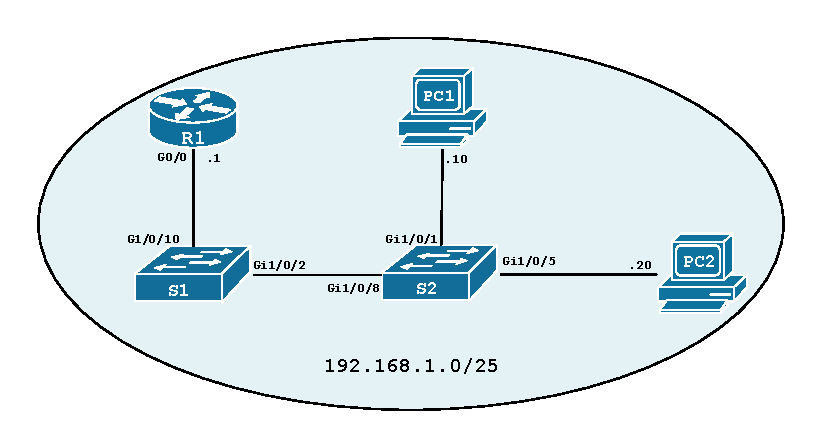
\includegraphics[width=\linewidth]{topology-2}
	\caption{Το σχέδιο της αναλυτικής τοπολογίας προς υλοποίηση.}\label{fig:topology2}
\end{figure}

\begin{IpAddressTable}{Σχήμα διευθυνσιοδότησης της τοπολογίας του πρώτου σεναρίου.}{addr2}
							 & Gi0/0		& 10.1.0.10		& 255.255.255.0			&\\
							 & \hl{Gi0/1}	& \hl{10.1.3.1} & \hl{255.255.255.0}	&\\
	\multirow{-3}{*}{R1}	 & loopback0	& 1.1.1.1		& 255.255.255.255		&\multirow{-3}{*}{1.1.1.1}\\
	\rowcolor{lightgray}	 & ether5		& 10.1.0.20		& 255.255.255.0 	    &\\
	\rowcolor{lightgray}	 & ether6		& 172.16.0.1	& 255.255.255.0			&\\
	\rowcolor{lightgray}	 & \hl{ether4}	& \hl{10.1.2.1}	& \hl{255.255.255.0}	&\\
	\rowcolor{lightgray}
	\multirow{-4}{*}{R2}	 & loopback0	& 2.2.2.2		& 255.255.255.255		&\multirow{-4}{*}{-} \\
							 & \hl{ether1} 	& \hl{10.1.2.2} & \hl{255.255.255.0}	&\\
							 & ether5		& 172.16.1.1	& 255.255.255.0			&\\
							 & \hl{ether6}	& \hl{10.1.3.2}& \hl{255.255.255.0}	&\\
	\multirow{-4}{*}{R3}	 & loopback0	& 3.3.3.3		& 255.255.255.255		& \multirow{-3}{*}{-} \\
	\rowcolor{lightgray}	 & Gi0/2		& 192.168.1.1	& 255.255.255.0 		& \\
	\rowcolor{lightgray}	 & Gi0/0		& 172.16.1.2	& 255.255.255.0 		& \\
	\rowcolor{lightgray}	 
	\multirow{-3}{*}{R4}	 & Gi0/1		& 172.16.0.2	& 255.255.255.0			& \multirow{-2}{*}{-}	\\
	PC1 	 				 & \NIC	  		& 192.168.1.2	& 255.255.255.0 		& 192.168.1.1
\end{IpAddressTable}
\newpage
%\begin{IpAddressTableNoDefaultRoute}{Σχήμα διευθυνσιοδότησης της τοπολογίας του δεύτερου σεναρίου.}{addr2}
%							R1	 	& Gi0/1		& 10.1.3.1 		& 255.255.255.0	 \\
%	\rowcolor{lightgray}	R2 		& Gi0/2 	& 10.1.2.2 		& 255.255.255.0	 \\
%									& ether1 	& 10.1.3.2 		& 255.255.255.0	 \\
%	\multirow{-2}{*}{R3}  			& ether6 	& 10.1.2.30 	& 255.255.255.0
%\end{IpAddressTableNoDefaultRoute}

Στο δεύτερο σενάριο θα εστιάσετε στον αλγόριθμο STP και στη διαδικασία υπολογισμού μονοπατιών του OSPF. Στόχος του σεναρίου είναι να αλλάξετε τα κόστη των διεπαφών ώστε να επηρεάσετε τον πίνακα δρομολόγησης του R1.

Αν έχετε υλοποιήσει ήδη την τοπολογία του πρώτου σεναρίου, τότε ακολουθήστε τις εξής οδηγίες για την προσαρμόσετε στη νέα τοπολογία:
\begin{itemize}
	\item Συνδέστε απευθείας τη διεπαφή Gi0/0 του R1 με τη διεπαφή ether5 του R2.
	\item Συνδέστε απευθείας τη διεπαφή ether4 του R2 με τη διεπαφή ether1 του R3. 
	\item Συνδέστε απευθείας τη διεπαφή Gi0/1 του R1 με τη διεπαφή ether6 του R3. 
	\item Εφαρμόστε \textbf{μόνο} τις νέες πληροφορίες διευθυνσιοδότησης που απεικονίζονται στον πίνακα \ref{tab:addr2} και έχουν κίτρινη επισύναψη.
	\item Διαφημίστε τα νέα δίκτυα της τοπολογίας (10.1.3.0/24 και 10.1.2.0/4) από τους δρομολογητές R1, R2 και R3.
\end{itemize}

\subsection{Αλλαγή της τιμής αναφοράς εύρους ζώνης}

Το Cisco IOS υπολογίζει αυτόματα το κόστος κάθε διεπαφής διαιρώντας μια τιμή αναφοράς με το εύρος ζώνης της διεπαφής. Δηλαδή:%
%
$$Cost = \dfrac{Reference\_Bandwidth}{Interface\_Bandwidth}$$

Από προεπιλογή, τιμή αναφοράς για το Cisco IOS είναι τα 100 Mbit/s, κάτι το οποίο σημαίνει ότι οι διεπαφές με ρυθμό μετάδοσης από 100 Mbit/s και πάνω έχουν κόστος 1. Αυτό το κριτήριο δεν είναι απόλυτα ρεαλιστικό, αφού γρηγορότερες ζεύξεις έχουν το ίδιο κόστος με τις πιο αργές, γιαυτό είναι καλή πρακτική η αλλαγή της προεπιλεγμένης τιμής αναφοράς.

Σε αντίθεση με το Cisco IOS, το RouterOS εφαρμόζει για όλες τις διεπαφές κόστος 10. 

Ξεκινώντας, καταγράψτε τον πίνακα δρομολόγησης του R1 πριν τις αλλαγές:

\begin{CommandBox}
R1#`\textbf{show ip route ospf | begin Gateway}`
Gateway of last resort is not set

      2.0.0.0/32 is subnetted, 1 subnets
O        2.2.2.2 [110/11] via 10.1.0.20, 01:24:08, GigabitEthernet0/0
      3.0.0.0/32 is subnetted, 1 subnets
O        3.3.3.3 [110/11] via 10.1.3.2, 00:18:59, GigabitEthernet0/1
      10.0.0.0/8 is variably subnetted, 5 subnets, 2 masks
O        10.1.2.0/24 [110/11] via 10.1.3.2, 00:00:51, GigabitEthernet0/1
                     [110/11] via 10.1.0.20, 00:51:33, GigabitEthernet0/0
      172.16.0.0/24 is subnetted, 2 subnets
O        172.16.0.0 [110/11] via 10.1.0.20, 01:23:57, GigabitEthernet0/0
O        172.16.1.0 [110/11] via 10.1.3.2, 00:18:59, GigabitEthernet0/1
O     192.168.1.0/24 [110/12] via 10.1.3.2, 00:18:59, GigabitEthernet0/1
                     [110/12] via 10.1.0.20, 01:23:57, GigabitEthernet0/0
\end{CommandBox}\vspace*{0.25cm}

Επίσης, επιβεβαιώστε ότι το κόστος των διεπαφών του R1 είναι το προεπιλεγμένο:

\begin{CommandBox}
R1#`\textbf{show ip ospf interface g0/0 | include Cost}`
  Process ID 1, Router ID 1.1.1.1, Network Type BROADCAST, `\hl{Cost: 1}`
  Topology-MTID    Cost    Disabled    Shutdown      Topology Name
R1#`\textbf{show ip ospf interface g0/1 | include Cost}`
  Process ID 1, Router ID 1.1.1.1, Network Type BROADCAST, `\hl{Cost: 1}`
  Topology-MTID    Cost    Disabled    Shutdown      Topology Name
\end{CommandBox}

Δώστε τις εξής εντολές στον R1 για να αλλάξετε την τιμή αναφοράς στα 10 Gbit/s. Αυτό σημαίνει ότι o δρομολογητής θα εφαρμόζει προεπιλεγμένο κόστος 1 στις διεπαφές 10 Gbit/s, κόστος 10 στις 1 Gbit/s κ.ο.κ:

\begin{CommandBox}
R1(config)# `\textbf{router ospf 1}`
R1(config-router)# `\textbf{auto-cost reference-bandwidth 10000}`
% OSPF: Reference bandwidth is changed.
        Please ensure reference bandwidth is consistent across all routers.
R1(config-router)#
\end{CommandBox}

Δώστε τις αντίστοιχες εντολές και στον R4. Δεν χρειάζεται να αλλάξετε τα κόστη για τους δρομολογητές MikroTik, αφού οι διεπαφές Gigabit θα έχουν το ίδιο κόστος με τις διεπαφές των δρομολογητών Cisco

Επιβεβαιώστε πως τα κόστη των διεπαφών έχουν αλλάξει με την κατάλληλη εντολή show. Ενδεικτικά:

\begin{CommandBox}
R1# `\textbf{show ip ospf interface g0/0 | include Cost}`
  Process ID 1, Router ID 1.1.1.1, Network Type BROADCAST, `\hl{Cost: 10}`
  Topology-MTID	Cost	Disabled	Shutdown	Topology Name
R1#
\end{CommandBox}

Οι αλλαγές διαδίδονται κατευθείαν στο δίκτυο, χωρίς επανεκκίνηση των διεργασιών OSPF. Έπειτα από μερικά δευτερόλεπτα προβάλλετε τον πίνακα δρομολόγησης του R1. Θα πρέπει να δείτε πως οι διαδρομές δεν έχουν αλλάξει, λόγω της τοποθεσίας των δρομολογητών MikroTik στο δίκτυο, έχουν αλλάξει όμως οι μετρικές τους.

{\small
\begin{CommandBox}
R1# `\textbf{show ip route ospf | begin Gateway}`
Gateway of last resort is not set

      2.0.0.0/32 is subnetted, 1 subnets
O        2.2.2.2 [110/`\hl{20}`] via 10.1.0.20, 00:03:07, GigabitEthernet0/0
      3.0.0.0/32 is subnetted, 1 subnets
O        3.3.3.3 [110/`\hl{20}`] via 10.1.3.2, 00:03:07, GigabitEthernet0/1
      10.0.0.0/8 is variably subnetted, 5 subnets, 2 masks
O        10.1.2.0/24 [110/`\hl{20}`] via 10.1.3.2, 00:03:07, GigabitEthernet0/1
                     [110/`\hl{20}`] via 10.1.0.20, 00:03:07, GigabitEthernet0/0
      172.16.0.0/24 is subnetted, 2 subnets
O        172.16.0.0 [110/`\hl{20}`] via 10.1.0.20, 00:03:07, GigabitEthernet0/0
O        172.16.1.0 [110/`\hl{20}`] via 10.1.3.2, 00:03:07, GigabitEthernet0/1
O     192.168.1.0/24 [110/`\hl{30}`] via 10.1.3.2, 00:00:19, GigabitEthernet0/1
                     [110/`\hl{30}`] via 10.1.0.20, 00:00:19, GigabitEthernet0/0

\end{CommandBox}}

\notebox{Παρατηρείτε στους πίνακες δρομολόγησης πως για τον ίδιο προορισμό υπάρχουν πολλαπλές διαδρομές. Όταν το OSPF υπολογίζει πολλές διαδρομές με το ίδιο ελάχιστο κόστος προς έναν προορισμό, τότε τις εγκαθιστά όλες στον πίνακα δρομολόγησης και εφαρμόζει εξισορρόπηση φόρτου (load balancing) μεταξύ των διαδρομών αυτών.}

\subsection{Χειροκίνητη αλλαγή του κόστους}
Υπάρχουν περιπτώσεις στις οποίες οι διαχειριστές ενός δικτύου έχουν λόγο να αλλάξουν χειροκίνητα το κόστος διέλευσης από μια διεπαφή. Για παράδειγμα, μπορεί ένα AS να έχει προτίμηση προς συγκεκριμένο πάροχο δικτύου ή να εφαρμόζεται χρέωση για τη χρήση της ζεύξης.

Θεωρήστε, λοιπόν, πως ο R1 θέλει να αποφύγει να χρησιμοποιεί τη ζεύξη του με τον R3 για να δρομολογεί πακέτα. Δώστε τις εντολές που ακολουθούν ώστε να αλλάξτε το κόστος της διεπαφής Gi0/1 του R1 σε 1500:

\begin{CommandBox}
R1(config)# `\textbf{interface gi0/1}`
R1(config-if)# `\textbf{ip ospf cost 1500}`
\end{CommandBox}

Παρατηρώντας τον πίνακα δρομολόγησης του R1 θα διαπιστώσετε πως πλέον ο δρομολογητής χρησιμοποιεί αποκλειστικά τη διεπαφή Gi0/0 για την επικοινωνία με το υπόλοιπο δίκτυο:

\begin{CommandBox}
R1# `\textbf{show ip route ospf | begin Gateway}`
Gateway of last resort is not set

      2.0.0.0/32 is subnetted, 1 subnets
O        2.2.2.2 [110/20] via 10.1.0.20, 00:16:00, GigabitEthernet0/0
      3.0.0.0/32 is subnetted, 1 subnets
O        3.3.3.3 [110/`\hl{30}`] via 10.1.0.20, 00:00:03, GigabitEthernet0/0
      10.0.0.0/8 is variably subnetted, 5 subnets, 2 masks
O        10.1.2.0/24 [110/20] via 10.1.0.20, 00:16:00, GigabitEthernet0/0
      172.16.0.0/24 is subnetted, 2 subnets
O        172.16.0.0 [110/20] via 10.1.0.20, 00:16:00, GigabitEthernet0/0
O        172.16.1.0 [110/30] via 10.1.0.20, 00:00:03, GigabitEthernet0/0
O     192.168.1.0/24 [110/30] via 10.1.0.20, 00:13:12, GigabitEthernet0/0
\end{CommandBox}\vspace*{0.25cm}

Τέλος, επαναφέρετε το αρχικό κόστος της διεπαφής με την εντολή:

\begin{CommandBox}
R1(config-if)# `\textbf{no ip ospf cost 1500}`
\end{CommandBox}

\newpage

\section{Σενάριο: Δρομολόγηση OSPFv2 μεταξύ περιοχών}

\begin{figure}[H]
	\centering
	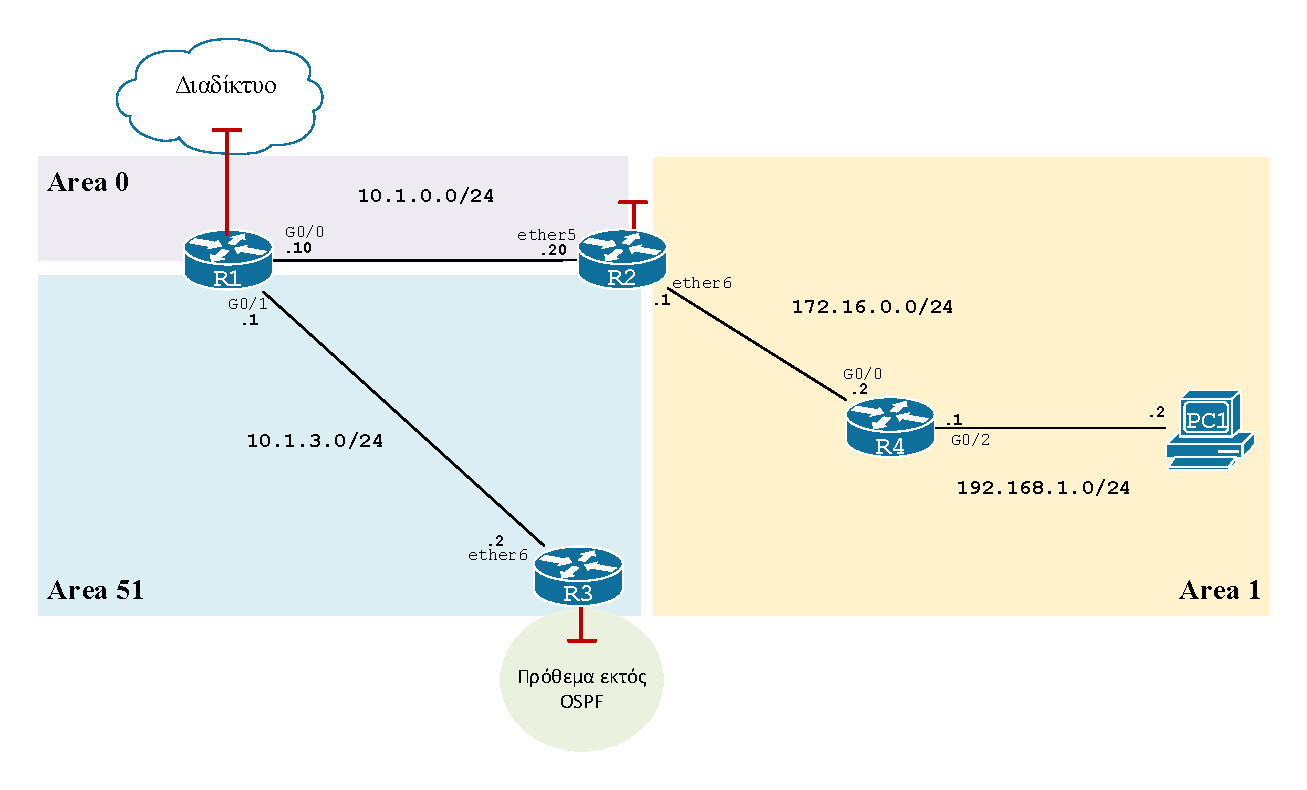
\includegraphics[width=\linewidth]{topology-3}
	\caption{Το σχέδιο της αναλυτικής τοπολογίας προς υλοποίηση.}\label{fig:topology3}
\end{figure}

\begin{IpAddressTable}{Σχήμα διευθυνσιοδότησης της τοπολογίας του τρίτου σεναρίου.}{addr3}
						 & Gi0/0		& 10.1.0.10		& 255.255.255.0			&\\
						 & Gi0/1		& 10.1.3.1 		& 255.255.255.0			&\\
\multirow{-3}{*}{R1}	 & loopback0	& 1.1.1.1		& 255.255.255.255		&\multirow{-3}{*}{1.1.1.1}\\
\rowcolor{lightgray}	 & ether5		& 10.1.0.20		& 255.255.255.0 	    &\\
\rowcolor{lightgray}	 & ether6		& 172.16.0.1	& 255.255.255.0			&\\
\rowcolor{lightgray}
\multirow{-3}{*}{R2}	 & loopback0	& 2.2.2.2		& 255.255.255.255		&\multirow{-3}{*}{-} \\
						 & ether6		& 10.1.3.2		& 255.255.255.0			&\\
\multirow{-2}{*}{R3}	 & loopback0	& 3.3.3.3		& 255.255.255.255		& \multirow{-2}{*}{-} \\
\rowcolor{lightgray}	 & Gi0/2		& 192.168.1.1	& 255.255.255.0 		& \\
\rowcolor{lightgray}	 
\multirow{-2}{*}{R4}	 & Gi0/0		& 172.16.1.2	& 255.255.255.0			& \multirow{-2}{*}{-}	\\
PC1 	 				 & \NIC	  		& 192.168.1.2	& 255.255.255.0 		& 192.168.1.1
\end{IpAddressTable}

Στο τρίτο σενάριο OSPF θα υλοποιήσετε πολλαπλές περιοχές OSPF, αναδιανέμοντας την προεπιλεγμένη πύλη και εξωτερικές διαδρομές. Ακόμη, θα ρυθμίσετε τις κανονικές περιοχές ως totally stub και totally NSSA με σκοπό να περιορίσετε τη διάδοση περιττών διαφημίσεων.

Αν έχετε ήδη υλοποιήσει την τοπολογία του προηγούμενου σεναρίου, τότε ακολουθήστε τις εξής οδηγίες για να την προσαρμόσετε στη νεα τοπολογία:
\begin{itemize}
	\item Αφαιρέστε το καλώδιο μεταξύ του R3 και του R4.
	\item Αφαιρέστε το καλώδιο μεταξύ του R2 και του R3.
	\item Αφαιρέστε όλα τα διαφημιζόμενα δίκτυα OSPF από όλους τους δρομολογητές. Για παράδειγμα, στον R1 και τον R3 μπορείτε να εκτελέσετε τις εξής εντολές:

\begin{CommandBox}
R1(config-router)#`\textbf{no router ospf 1}`
\end{CommandBox}

\begin{CommandBox}
[admin@R3] > `\textbf{routing ospf network print}`
Flags: X - disabled, I - invalid
`\begin{tabular}{lll}
	\#   &NETWORK            &AREA\\
	0   &10.1.3.0/24        &backbone\\
	1   &10.1.2.0/24        &backbone\\
	2   &172.16.1.0/24      &backbone\\
	3   &3.3.3.3/32         &backbone
\end{tabular}`
[admin@R3] > `\textbf{routing ospf network remove 0,1,2,3}`
\end{CommandBox}
\end{itemize}

Πριν ξεκινήσετε την υλοποίηση, καταγράψτε στον πίνακα \ref{tab:categories} το είδος του κάθε δρομολογητή, σύμφωνα με το σχήμα τοπολογίας \ref{fig:topology3}:

\begin{table}[ht]\renewcommand\arraystretch{1.5}
	\centering	\rowcolors{2}{lightgray}{white}	
	\begin{tabular}{lccc}\FormatFirstRow
		\textbf{Δρομολογητής}	& \textbf{Εσωτερικός}	& \textbf{ABR}	& \textbf{ASBR} \\
		\textbf{R1}				&\radioButton{a}{10bp}{10bp}{1} & \radioButton{a}{10bp}{10bp}{2} & \radioButton{a}{10bp}{10bp}{3}\\
		\textbf{R2}			    &\radioButton{b}{10bp}{10bp}{4} & \radioButton{b}{10bp}{10bp}{5} & \radioButton{b}{10bp}{10bp}{6}\\
		\textbf{R3}				&\radioButton{c}{10bp}{10bp}{9} & \radioButton{c}{10bp}{10bp}{7} & \radioButton{c}{10bp}{10bp}{8}\\
		\textbf{R4}				&\radioButton{d}{10bp}{10bp}{10} & \radioButton{d}{10bp}{10bp}{211} & \radioButton{d}{10bp}{10bp}{13}\\
	\end{tabular}	
	\caption{Οι ρόλοι των δρομολογητών της τρίτης τοπολογίας.}\label{tab:categories}
\end{table}

\notebox{Λόγω της υλοποίησης αρχιτεκτονικής περιοχών ήταν υποχρεωτική η αφαίρεση της σύνδεσης του R3 με τον R4, διότι μια από τις αρχές του OSPF πολλών περιοχών είναι ότι η κίνηση που προορίζεται προς περιοχή non-backbone πρέπει απαραίτητα να διασχίζει την περιοχή κορμού.}

\subsection{Ρύθμιση πολλαπλών περιοχών για Cisco IOS}

Ξεκινώντας με τον R1, παρατηρείτε πως ο δρομολογητής έχει διεπαφές σε δυο περιοχές, την 0 και την 51. Διαφημίστε, λοιπόν, τα αντίστοιχα δίκτυα των διεπαφών δίνοντας τις εξής εντολές:

\begin{CommandBox}
R1(config)#`\textbf{router ospf 1}`
R1(config-router)#`\textbf{network 10.1.0.0 0.0.0.255 area 0}`
R1(config-router)#`\textbf{network 10.1.3.0 0.0.0.255 area 51}`
R1(config-router)#
\end{CommandBox}

Δώστε αντίστοιχες εντολές στον δρομολογητή R4, ρυθμίζοντας παράλληλα τη διεπαφή Gi0/2 ως passive.

\subsection{Ρύθμιση πολλαπλών περιοχών για RouterOS}

Για τους δρομολογητές MikroTik θα χρειαστεί να προσθέσετε στον υποκατάλογο \texttt{/routing ospf area} τις περιοχές που θα χρησιμοποιήσει ο κάθε δρομολογητής και έπειτα να προσαρτήσετε τα δίκτυα OSPF σε αυτές τις περιοχές. 

Για την παραμετροποίηση του R2 δώστε τις ακόλουθες εντολές:

\begin{CommandBox}
[admin@R2] > `\textbf{routing ospf area add name=area1 area-id=0.0.0.1}`
[admin@R2] > `\textbf{routing ospf network add network=10.1.0.0/24 area=backbone}`
[admin@R2] > `\textbf{routing ospf network add network=172.16.0.0/24 area=area1}`
[admin@R2] >
\end{CommandBox}

\subsection{Αναδιανομή προεπιλεγμένης πύλης}
Όπως φαίνεται στο σχήμα της τοπολογίας, ο R1 αποτελεί το σημείο πρόσβασης του δικτύου OSPF στο Διαδίκτυο. Πρακτικά, αυτό σημαίνει πως ο R1 έχει τον ρόλο ASBR και ότι είναι ο μοναδικός δρομολογητής που διαχέει στο δίκτυο OSPF την πληροφορία προεπιλεγμένης πύλης που οδηγεί στο Διαδίκτυο.

Έχοντας ήδη ρυθμίσει την προεπιλεγμένη πύλη στον R1, αρκεί να δώσετε την εξής εντολή για να ενεργοποιήσετε τη διάδοση προεπιλεγμένης πύλης:

\begin{CommandBox}
R1(config-router)#`\textbf{default-information originate}`
\end{CommandBox}

\subsection{Επιβεβαίωση ρυθμίσεων}

Αφού περάσουν μερικά δευτερόλεπτα ώστε να συγκλίνει το δίκτυο, παρατηρήστε τον πίνακα δρομολόγησης του R4 και του R3:

\begin{CommandBox}
R4#`\textbf{show ip route | begin Gateway}`
`\hl{Gateway of last resort is 172.16.0.1 to network 0.0.0.0}`

`\hl{O*E2}`  `\hl{0.0.0.0/0 [110/1] via 172.16.0.1, 00:10:48, GigabitEthernet0/0}`
      10.0.0.0/24 is subnetted, 2 subnets
`\hl{O IA}`     `\hl{10.1.0.0 [110/20] via 172.16.0.1, 00:01:02, GigabitEthernet0/0}`
`\hl{O IA}`     `\hl{10.1.3.0 [110/30] via 172.16.0.1, 00:00:33, GigabitEthernet0/0}`
      172.16.0.0/16 is variably subnetted, 2 subnets, 2 masks
C        172.16.0.0/24 is directly connected, GigabitEthernet0/0
L        172.16.0.2/32 is directly connected, GigabitEthernet0/0
      192.168.1.0/24 is variably subnetted, 2 subnets, 2 masks
C        192.168.1.0/24 is directly connected, GigabitEthernet0/2
L        192.168.1.1/32 is directly connected, GigabitEthernet0/2
R4#
\end{CommandBox}

\begin{CommandBox}
[admin@R3] > routing ospf route print
 # DST-ADDRESS        STATE          COST       GATEWAY        INTERFACE
 0 0.0.0.0/0          ext-2          1          10.1.3.1       ether6
 1 10.1.0.0/24        inter-area     20         10.1.3.1       ether6
 2 10.1.3.0/24        intra-area     10         0.0.0.0        ether6
 3 172.16.0.0/24      inter-area     30         10.1.3.1       ether6
 4 192.168.1.0/24     inter-area     40         10.1.3.1       ether6
[admin@R3] >
\end{CommandBox}  

Αποτέλεσμα της αρχιτεκτονικής περιοχών είναι ότι οι ABR διαφημίζουν τα δίκτυα άλλων περιοχών σε LSA τύπου 3, οι διαδρομές των οποίων απεικονίζονται ως \ip{O IA} ή \ip{inter-area} στον πίνακα δρομολόγησης. 

Συμπληρωματικά, μπορείτε να δείτε και την LSDB των δρομολογητών, η οποία διατηρεί πίνακα με LSA τύπου 1, 2 και 3 για κάθε περιοχή στην οποία συμμετέχει ο δρομολογητής. Παρατηρείτε πως το πλήθος των LSA τύπου 1 και 2 μειώθηκε, οι διαδρομές που οδηγούν σε άλλες περιοχές υπάρχουν στη βάση ως LSA τύπου 3, και η προεπιλεγμένη πύλη υπάρχει στη βάση ως LSA τύπου 5. Ακόμη, διακρίνεται και η ταυτότητα του ASBR ως LSA τύπου 4.

\begin{CommandBox}
R4#`\textbf{show ip ospf database}`

            OSPF Router with ID (192.168.1.1) (Process ID 1)

                Router Link States (Area 1)      `\hl{Type-1 LSA}`

Link ID         ADV Router      Age         Seq#       Checksum Link count
2.2.2.2         2.2.2.2         645         0x80000002 0x00605B 1
192.168.1.1     192.168.1.1     644         0x80000003 0x0094CC 2

                Net Link States (Area 1)         `\hl{Type-2 LSA}`

Link ID         ADV Router      Age         Seq#       Checksum
172.16.0.2      192.168.1.1     644         0x80000001 0x00EEAD

                Summary Net Link States (Area 1)   `\hl{Type-3 LSA}`

Link ID         ADV Router      Age         Seq#       Checksum
10.1.0.0        2.2.2.2         652         0x80000001 0x00053B
10.1.3.0        2.2.2.2         652         0x80000001 0x00ED4E

                Summary ASB Link States (Area 1)    `\hl{Type-4 LSA}`

Link ID         ADV Router      Age         Seq#       Checksum
1.1.1.1         2.2.2.2         310         0x80000001 0x0057EE

                `\hl{Type-5 AS}` External Link States

Link ID         ADV Router      Age         Seq#       Checksum Tag
0.0.0.0         1.1.1.1         271         0x80000001 0x001D91 1
R4#
\end{CommandBox}

\begin{CommandBox}
[admin@R3] > routing ospf lsa print
AREA      TYPE         ID            ORIGINATOR  SEQUENCE-NUMBER     AGE
area51    router       1.1.1.1       1.1.1.1          0x80000003     512
area51    router       3.3.3.3       3.3.3.3          0x80000002     651
area51    network      10.1.3.1      1.1.1.1          0x80000001     652
area51    `\hl{summary-n... 10.1.0.0}`      `\hl{1.1.1.1}`          0x80000001    1105
area51    `\hl{summary-n... 172.16.0.0}`    `\hl{1.1.1.1}`          0x80000001     846
area51    `\hl{summary-n... 192.168.1.0}`   `\hl{1.1.1.1}`          0x80000001     843
`\hl{external}`  `\hl{as-external}`  `\hl{0.0.0.0}`       `\hl{1.1.1.1}`          0x80000001     470
[admin@R3] >
\end{CommandBox}

\subsection{Περιοχές NSSA και stub}

Η LSDB και ο πίνακας δρομολόγησης μεγεθύνονται σημαντικά, για κάθε περιοχή στην οποία συμμετέχει ένας δρομολογητής και για κάθε εξωτερικό δίκτυο που διαφημίζεται. Διαπιστώνει κάποιος πως για τους δρομολογητές R3 και R4, η μεμονωμένη διαφήμιση κάθε δικτύου από άλλες περιοχές OSPF σε LSA τύπου 5 είναι περιττή και θα μπορούσε να εμποδιστεί, αφού οι εν λόγω δρομολογητές θα μπορούσαν να χρησιμοποιήσουν ως προεπιλεγμένη πύλη τον ABR που τους εξυπηρετεί για να προωθήσουν κίνηση που προορίζεται είτε προς άλλες περιοχές είτε προς το Διαδίκτυο. Αυτή τη λειτουργία εξυπηρετούν οι περιοχές totally stub, οι οποίες αντικαθιστούν τα LSA τύπου 3, 4 και 5 με διάδοση προεπιλεγμένης πύλης.

\subsubsection*{Ορισμός της περιοχής 1 ως totally stub}

Ξεκινώντας από την περιοχή 1, θα πρέπει να ορίσετε την περιοχή ως totally stub σε όλους τους δρομολογητές που ανήκουν σε αυτήν. Στον R4 δώστε τις εξής εντολές:

\begin{CommandBox}
R4(config)#`\textbf{router ospf 1}`
R4(config-router)#`\textbf{area 1 stub no-summary}`
\end{CommandBox}

Αντίστοιχα για τον δρομολογητή R2:

\begin{CommandBox}
[admin@R2] > `\textbf{routing ospf area set area1 type=stub inject-summary-lsas=no}`
\end{CommandBox}

\subsubsection*{Ορισμός της περιοχής 51 ως totally NSSA}

Η περιοχή 51 δεν μπορεί να οριστεί ως stub, διότι ο R3 επιθυμεί να διαδίδει στο δίκτυο OSPF ένα πρόθεμα που δεν ανήκει στο δίκτυο OSPF, δηλαδή να στέλνει LSA τύπου 5, ενώ ταυτόχρονα δεν θέλει να λαμβάνει LSA τύπου 3, 4 και 5 για άλλα δίκτυα. Την ευελιξία αυτή προσφέρει η περιοχή totally NSSA.

Για τον R1 δώστε την εξής εντολή, ώστε να μετατρέψετε την περιοχή 51 σε totally NSSA. Πρόσθετα, χρειάζεται να ενεργοποιήσετε ρητά τη μετάφραση LSA τύπου 7 σε τύπου 5.

\begin{CommandBox}
R1(config)#`\textbf{router ospf 1}`
R1(config-router)#`\textbf{area 51 nssa no-summary}`
R1(config-router)#`\textbf{area 51 nssa translate type7 always}`
\end{CommandBox}
 
Στον R3 ρυθμίστε την ίδια περιοχή ως Totally NSSA και διαφημίστε το δίκτυο βρόχου στην περιοχή αυτή:

\begin{CommandBox}
[admin@R3] > `\textbf{routing ospf area set 1 type=nssa inject-summary-lsas=no}`
[admin@R3] > `\textbf{routing ospf instance set 0 redistribute-connected=as-type-2}`
\end{CommandBox}

\subsection{Επιβεβαίωση ρυθμίσεων}

Προβάλλοντας τον πίνακα δρομολόγησης και την LSDB του R4, βλέπετε πως έχουν αφαιρεθεί οι διαδρομές των LSA τύπου 3 και 5. Οι διαδρομές αυτές έχουν αντικατασταθεί από την προεπιλεγμένη πύλη, η οποία εισάγεται στην LSDB και στον πίνακα δρομολόγησης ως LSA τύπου 3. 

\begin{CommandBox}
R4#`\textbf{sh ip route | begin Gateway}`
Gateway of last resort is 172.16.0.1 to network 0.0.0.0

`\hl{O*IA}`  `\hl{0.0.0.0/0 [110/11] via 172.16.0.1, 00:04:23, GigabitEthernet0/0}`
      172.16.0.0/16 is variably subnetted, 2 subnets, 2 masks
C        172.16.0.0/24 is directly connected, GigabitEthernet0/0
L        172.16.0.2/32 is directly connected, GigabitEthernet0/0
      192.168.1.0/24 is variably subnetted, 2 subnets, 2 masks
C        192.168.1.0/24 is directly connected, GigabitEthernet0/2
L        192.168.1.1/32 is directly connected, GigabitEthernet0/2
R4#
\end{CommandBox}

\begin{CommandBox}
R4#`\textbf{show ip ospf database}`

            OSPF Router with ID (192.168.1.1) (Process ID 1)

                Router Link States (Area 1)

Link ID         ADV Router      Age         Seq#       Checksum Link count
2.2.2.2         2.2.2.2         325         0x80000008 0x007245 1
192.168.1.1     192.168.1.1     472         0x80000008 0x005AF1 2

                Net Link States (Area 1)

Link ID         ADV Router      Age         Seq#       Checksum
172.16.0.2      192.168.1.1     472         0x80000002 0x000B92

                `\hl{Summary Net}` Link States (Area 1)

Link ID         ADV Router      Age         Seq#       Checksum
`\hl{0.0.0.0}`         `\hl{2.2.2.2}`         330         0x80000003 0x005301
R4#
\end{CommandBox}

Αντίστοιχα και για τον R3 παρατηρείτε πως λαμβάνει την προεπιλεγμένη πύλη ως LSA τύπου 3, ενώ παράλληλα εισάγει το πρόθεμα 3.3.3.3 ως εξωτερική διαδρομή τύπου 2 και το διαφημίζει ως LSA τύπου 7:

\begin{CommandBox}
[admin@R3] > `\textbf{routing ospf lsa print}`
AREA      TYPE         ID          ORIGINATOR   SEQUENCE-NUMBER      AGE
area51    router       1.1.1.1     1.1.1.1           0x80000008     1659
area51    router       3.3.3.3     3.3.3.3           0x80000007     1580
area51    network      10.1.3.1    1.1.1.1           0x80000001     1659
`\hl{area51}`    `\hl{summary-n... 0.0.0.0}`     1.1.1.1           0x80000003     1722
`\hl{area51}`    `\hl{type-7}`       `\hl{3.3.3.3}`     3.3.3.3           0x80000001     1580
\end{CommandBox}

\begin{CommandBox}
[admin@R3] > `\textbf{routing ospf route print}`
# DST-ADDRESS        STATE          COST       GATEWAY         INTERFACE
`\hl{0 0.0.0.0/0}`          `\hl{inter-area}`     11         10.1.3.1        ether6
`\hl{1 3.3.3.3/32}`         `\hl{imported-ext-2}` 20
2 10.1.3.0/24        intra-area     10         0.0.0.0         ether6
[admin@R3] >
\end{CommandBox}

Μπορείτε να επιβεβαιώσετε πως το πρόθεμα του R3 διαδίδεται αρχικά ως LSA τύπου 7 παρατηρώντας τον πίνακα δρομολόγησης και την LSDB του R1:

\begin{CommandBox}
R1#`\textbf{sh ip route ospf | begin Gateway}`
`\hl{Gateway of last resort is 0.0.0.0 to network 0.0.0.0}`

      3.0.0.0/32 is subnetted, 1 subnets
`\hl{O N2}`     `\hl{3.3.3.3 [110/20] via 10.1.3.2, 00:26:50, GigabitEthernet0/1}`
      172.16.0.0/24 is subnetted, 1 subnets
O IA     172.16.0.0 [110/20] via 10.1.0.20, 00:08:11, GigabitEthernet0/0
O IA  192.168.1.0/24 [110/30] via 10.1.0.20, 00:08:11, GigabitEthernet0/0
\end{CommandBox}

\begin{CommandBox}
R1#`\textbf{sh ip ospf database}`

            OSPF Router with ID (1.1.1.1) (Process ID 1)

                Router Link States (Area 0)

Link ID         ADV Router      Age         Seq#       Checksum Link count
1.1.1.1         1.1.1.1         974         0x80000007 0x00F8F5 1
2.2.2.2         2.2.2.2         510         0x80000009 0x0011EB 1

                Net Link States (Area 0)

Link ID         ADV Router      Age         Seq#       Checksum
10.1.0.10       1.1.1.1         1971        0x80000003 0x001102

                Summary Net Link States (Area 0)

Link ID         ADV Router      Age         Seq#       Checksum
10.1.3.0        1.1.1.1         974         0x80000004 0x001A04
172.16.0.0      2.2.2.2         589         0x80000004 0x000883
192.168.1.0     2.2.2.2         508         0x80000003 0x00379D

                Router Link States (Area 51)

Link ID         ADV Router      Age         Seq#       Checksum Link count
1.1.1.1         1.1.1.1         1708        0x80000008 0x0036AD 1
3.3.3.3         3.3.3.3         1630        0x80000007 0x005CA8 1

                Net Link States (Area 51)

Link ID         ADV Router      Age         Seq#       Checksum
10.1.3.1        1.1.1.1         1708        0x80000001 0x0026EA

                Summary Net Link States (Area 51)

Link ID         ADV Router      Age         Seq#       Checksum
0.0.0.0         1.1.1.1         1771        0x80000003 0x001719

                `\hl{Type-7 AS External}` Link States (Area 51)

Link ID         ADV Router      Age         Seq#       Checksum Tag
`\hl{3.3.3.3}`         `\hl{3.3.3.3}`         1630        0x80000001 0x00EF9C 0

                Type-5 AS External Link States

Link ID         ADV Router      Age         Seq#       Checksum Tag
0.0.0.0         1.1.1.1         1729        0x80000003 0x001993 1
3.3.3.3         1.1.1.1         1623        0x80000001 0x00FC83 0
R1#
\end{CommandBox}

Επίσης, ο R2 πρέπει να λαμβάνει το πρόθεμα 3.3.3.3 ως LSA τύπου 5:

\begin{CommandBox}
[admin@R2] > routing ospf lsa print
AREA        TYPE         ID            ORIGINATOR SEQUENCE-NUMBER    AGE
backbone    router       1.1.1.1       1.1.1.1         0x80000008     11
backbone    router       2.2.2.2       2.2.2.2         0x80000009   1579
backbone    network      10.1.0.10     1.1.1.1         0x80000004   1036
backbone    summary-n... 10.1.3.0      1.1.1.1         0x80000005     11
backbone    summary-n... 172.16.0.0    2.2.2.2         0x80000004   1657
backbone    summary-n... 192.168.1.0   2.2.2.2         0x80000003   1576
area1       router       2.2.2.2       2.2.2.2         0x80000008   1579
area1       router       192.168.1.1   192.168.1.1     0x80000008   1727
area1       network      172.16.0.2    192.168.1.1     0x80000002   1727
area1       summary-n... 0.0.0.0       2.2.2.2         0x80000003   1584
external    as-external  0.0.0.0       1.1.1.1         0x80000004    774
`\hl{external}`    `\hl{as-external}`  `\hl{3.3.3.3}`       `\hl{1.1.1.1}`         0x80000002    774
[admin@R2] >
\end{CommandBox}

Δοκιμάστε από τον PC1 να κάνετε \ip{ping} προς τις διευθύνσεις 1.1.1.1 και 3.3.3.3. Θα πρέπει οι εντολές να εκτελεστούν με επιτυχία. 

\newpage

\section{Αντιμετώπιση προβλημάτων\label{sec:tro}}
Στους πίνακες \ref{tab:tro-ios} και \ref{tab:tro-routeros} παρατίθενται οι εντολές που μπορούν να χρησιμοποιηθούν στο Cisco IOS και στο RouterOS για διάγνωση και αντιμετώπιση προβλημάτων.  

\begin{CommandTable}{Εντολές IOS για διάγνωση και αντιμετώπιση προβλημάτων}{tro-ios}
	Router\# \textbf{show ip protocols}			& Προβάλλονται γενικές πληροφορίες, όπως ο αριθμός διεργασίας, το router ID και τα διαφημιζόμενα δίκτυα.\\
	Router\# \textbf{show ip ospf neighbor}		& Προβάλλονται οι γείτονες, η κατάσταση της γειτνίασης και η διεπαφή μέσω της οποίας ο δρομολογητής επικοινωνεί με τον κάθε γείτονα.\\
	Router\# \textbf{show ip ospf interface}	& Προβάλλονται πληροφορίες για τις παραμετροποιήσεις OSPF ανά διεπαφή. Σε αυτές περιλαμβάνεται η περιοχή στην οποία ανήκει η κάθε διεπαφή, το κόστος διάσχισης και οι τιμές των χρονομέτρων.\\
	Router\# \textbf{show ip ospf database}		& Εμφανίζεται ολόκληρη η LSDB του δρομολογητή\\  
	Router\# \textbf{show ip ospf}				& Προβάλλονται γενικές πληροφορίες που αφορούν το OSPF.\\
	
	Router\# \textbf{clear ip ospf} [process-id] \textbf{process}			& Επαναφέρει τη διεργασία OSPF και τις γειτνιάσεις για συγκεκριμένη διεργασία 
\end{CommandTable}

\begin{CommandTable}{Εντολές RouterOS για διάγνωση και αντιμετώπιση προβλημάτων}{tro-routeros}
	{[admin@R2]} > \textbf{routing ospf neighbor print} 	& Προβάλλονται αναλυτικές πληροφορίες για τους γείτονες OSPF.\\
	{[admin@R2]} > \textbf{routing ospf interface print}	& Προβάλλονται αναλυτικές πληροφορίες για τις διεπαφές στις οποίες έχει ενεργοποιηθεί το OSPF.\\
	{[admin@R2]} > \textbf{routing ospf route print}		& Εμφανίζεται η RIB του OSPF.\\
	{[admin@R2]} > \textbf{routing ospf lsa print}			& Εμφανίζεται ολόκληρη η LSDB του δρομολογητή.\\
	{{[admin@R2]}~>~\textbf{routing~ospf~instance~disable~0}} {{[admin@R2]}~>~\textbf{routing~ospf~instance~enable~0}}		& Για απενεργοποίηση και επανενεργοποίηση της προεπιλεγμένης διεργασίας OSPF.\\
\end{CommandTable}


\end{document}
